\documentclass[11pt,a4paper, d]{scrartcl}
    \usepackage[scaled]{helvet}
    \usepackage{fancyhdr}
    \usepackage{amsmath}
\usepackage{amsthm}
\usepackage{amssymb}
\usepackage{amsfonts}
    \usepackage[breakable]{tcolorbox}
    \usepackage{parskip} % Stop auto-indenting (to mimic markdown behaviour)

    \usepackage{parskip} % Stop auto-indenting (to mimic markdown behaviour)
    
    \usepackage{iftex}
    \ifPDFTeX
    	\usepackage[T1]{fontenc}
    	\usepackage{mathpazo}
    \else
    	\usepackage{fontspec}
    \fi

    % Basic figure setup, for now with no caption control since it's done
    % automatically by Pandoc (which extracts ![](path) syntax from Markdown).
    \usepackage{graphicx}
     \graphicspath{{figures/}{RareEvent/figures/}}
    % Maintain compatibility with old templates. Remove in nbconvert 6.0
    \let\Oldincludegraphics\includegraphics
    % Ensure that by default, figures have no caption (until we provide a
    % proper Figure object with a Caption API and a way to capture that
    % in the conversion process - todo).
    \usepackage{caption}
    \DeclareCaptionFormat{nocaption}{}
    \captionsetup{format=nocaption,aboveskip=0pt,belowskip=0pt}

    \usepackage{float}
    \floatplacement{figure}{H} % forces figures to be placed at the correct location
    \usepackage{xcolor} % Allow colors to be defined
    \usepackage{enumerate} % Needed for markdown enumerations to work
    \usepackage{geometry} % Used to adjust the document margins
    \usepackage{amsmath} % Equations
    \usepackage{amssymb} % Equations
    \usepackage{textcomp} % defines textquotesingle
    % Hack from http://tex.stackexchange.com/a/47451/13684:
    \AtBeginDocument{%
        \def\PYZsq{\textquotesingle}% Upright quotes in Pygmentized code
    }
    \usepackage{upquote} % Upright quotes for verbatim code
    \usepackage{eurosym} % defines \euro
    \usepackage[mathletters]{ucs} % Extended unicode (utf-8) support
    \usepackage{fancyvrb} % verbatim replacement that allows latex
    \usepackage{grffile} % extends the file name processing of package graphics 
                         % to support a larger range
    \makeatletter % fix for old versions of grffile with XeLaTeX
    \@ifpackagelater{grffile}{2019/11/01}
    {
      % Do nothing on new versions
    }
    {
      \def\Gread@@xetex#1{%
        \IfFileExists{"\Gin@base".bb}%
        {\Gread@eps{\Gin@base.bb}}%
        {\Gread@@xetex@aux#1}%
      }
    }
    \makeatother
    \usepackage[Export]{adjustbox} % Used to constrain images to a maximum size
    \adjustboxset{max size={0.9\linewidth}{0.9\paperheight}}

    % The hyperref package gives us a pdf with properly built
    % internal navigation ('pdf bookmarks' for the table of contents,
    % internal cross-reference links, web links for URLs, etc.)
    \usepackage{hyperref}
    % The default LaTeX title has an obnoxious amount of whitespace. By default,
    % titling removes some of it. It also provides customization options.
    \usepackage{titling}
    \usepackage{longtable} % longtable support required by pandoc >1.10
    \usepackage{booktabs}  % table support for pandoc > 1.12.2
    \usepackage[inline]{enumitem} % IRkernel/repr support (it uses the enumerate* environment)
    \usepackage[normalem]{ulem} % ulem is needed to support strikethroughs (\sout)
                                % normalem makes italics be italics, not underlines
    \usepackage{mathrsfs}
    

    
    % Colors for the hyperref package
    \definecolor{urlcolor}{rgb}{0,.145,.698}
    \definecolor{linkcolor}{rgb}{.71,0.21,0.01}
    \definecolor{citecolor}{rgb}{.12,.54,.11}

    % ANSI colors
    \definecolor{ansi-black}{HTML}{3E424D}
    \definecolor{ansi-black-intense}{HTML}{282C36}
    \definecolor{ansi-red}{HTML}{E75C58}
    \definecolor{ansi-red-intense}{HTML}{B22B31}
    \definecolor{ansi-green}{HTML}{00A250}
    \definecolor{ansi-green-intense}{HTML}{007427}
    \definecolor{ansi-yellow}{HTML}{DDB62B}
    \definecolor{ansi-yellow-intense}{HTML}{B27D12}
    \definecolor{ansi-blue}{HTML}{208FFB}
    \definecolor{ansi-blue-intense}{HTML}{0065CA}
    \definecolor{ansi-magenta}{HTML}{D160C4}
    \definecolor{ansi-magenta-intense}{HTML}{A03196}
    \definecolor{ansi-cyan}{HTML}{60C6C8}
    \definecolor{ansi-cyan-intense}{HTML}{258F8F}
    \definecolor{ansi-white}{HTML}{C5C1B4}
    \definecolor{ansi-white-intense}{HTML}{A1A6B2}
    \definecolor{ansi-default-inverse-fg}{HTML}{FFFFFF}
    \definecolor{ansi-default-inverse-bg}{HTML}{000000}

    % common color for the border for error outputs.
    \definecolor{outerrorbackground}{HTML}{FFDFDF}

    % commands and environments needed by pandoc snippets
    % extracted from the output of `pandoc -s`
    \providecommand{\tightlist}{%
      \setlength{\itemsep}{0pt}\setlength{\parskip}{0pt}}
    \DefineVerbatimEnvironment{Highlighting}{Verbatim}{commandchars=\\\{\}}
    % Add ',fontsize=\small' for more characters per line
    \newenvironment{Shaded}{}{}
    \newcommand{\KeywordTok}[1]{\textcolor[rgb]{0.00,0.44,0.13}{\textbf{{#1}}}}
    \newcommand{\DataTypeTok}[1]{\textcolor[rgb]{0.56,0.13,0.00}{{#1}}}
    \newcommand{\DecValTok}[1]{\textcolor[rgb]{0.25,0.63,0.44}{{#1}}}
    \newcommand{\BaseNTok}[1]{\textcolor[rgb]{0.25,0.63,0.44}{{#1}}}
    \newcommand{\FloatTok}[1]{\textcolor[rgb]{0.25,0.63,0.44}{{#1}}}
    \newcommand{\CharTok}[1]{\textcolor[rgb]{0.25,0.44,0.63}{{#1}}}
    \newcommand{\StringTok}[1]{\textcolor[rgb]{0.25,0.44,0.63}{{#1}}}
    \newcommand{\CommentTok}[1]{\textcolor[rgb]{0.38,0.63,0.69}{\textit{{#1}}}}
    \newcommand{\OtherTok}[1]{\textcolor[rgb]{0.00,0.44,0.13}{{#1}}}
    \newcommand{\AlertTok}[1]{\textcolor[rgb]{1.00,0.00,0.00}{\textbf{{#1}}}}
    \newcommand{\FunctionTok}[1]{\textcolor[rgb]{0.02,0.16,0.49}{{#1}}}
    \newcommand{\RegionMarkerTok}[1]{{#1}}
    \newcommand{\ErrorTok}[1]{\textcolor[rgb]{1.00,0.00,0.00}{\textbf{{#1}}}}
    \newcommand{\NormalTok}[1]{{#1}}
    
    % Additional commands for more recent versions of Pandoc
    \newcommand{\ConstantTok}[1]{\textcolor[rgb]{0.53,0.00,0.00}{{#1}}}
    \newcommand{\SpecialCharTok}[1]{\textcolor[rgb]{0.25,0.44,0.63}{{#1}}}
    \newcommand{\VerbatimStringTok}[1]{\textcolor[rgb]{0.25,0.44,0.63}{{#1}}}
    \newcommand{\SpecialStringTok}[1]{\textcolor[rgb]{0.73,0.40,0.53}{{#1}}}
    \newcommand{\ImportTok}[1]{{#1}}
    \newcommand{\DocumentationTok}[1]{\textcolor[rgb]{0.73,0.13,0.13}{\textit{{#1}}}}
    \newcommand{\AnnotationTok}[1]{\textcolor[rgb]{0.38,0.63,0.69}{\textbf{\textit{{#1}}}}}
    \newcommand{\CommentVarTok}[1]{\textcolor[rgb]{0.38,0.63,0.69}{\textbf{\textit{{#1}}}}}
    \newcommand{\VariableTok}[1]{\textcolor[rgb]{0.10,0.09,0.49}{{#1}}}
    \newcommand{\ControlFlowTok}[1]{\textcolor[rgb]{0.00,0.44,0.13}{\textbf{{#1}}}}
    \newcommand{\OperatorTok}[1]{\textcolor[rgb]{0.40,0.40,0.40}{{#1}}}
    \newcommand{\BuiltInTok}[1]{{#1}}
    \newcommand{\ExtensionTok}[1]{{#1}}
    \newcommand{\PreprocessorTok}[1]{\textcolor[rgb]{0.74,0.48,0.00}{{#1}}}
    \newcommand{\AttributeTok}[1]{\textcolor[rgb]{0.49,0.56,0.16}{{#1}}}
    \newcommand{\InformationTok}[1]{\textcolor[rgb]{0.38,0.63,0.69}{\textbf{\textit{{#1}}}}}
    \newcommand{\WarningTok}[1]{\textcolor[rgb]{0.38,0.63,0.69}{\textbf{\textit{{#1}}}}}
    
    
    % Define a nice break command that doesn't care if a line doesn't already
    % exist.
    \def\br{\hspace*{\fill} \\* }
    % Math Jax compatibility definitions
    \def\gt{>}
    \def\lt{<}
    \let\Oldtex\TeX
    \let\Oldlatex\LaTeX
    \renewcommand{\TeX}{\textrm{\Oldtex}}
    \renewcommand{\LaTeX}{\textrm{\Oldlatex}}
    % Document parameters
    % Document title
  \rhead{\begin{picture}(0,0)(0,0)\put(53,-62){
\includegraphics[height=4cm]{logoR}}\end{picture}}
\lhead{Handout - Dynamical Systems}
\lfoot{File: \jobname, date: \today}
\rfoot{Page \thepage}

\author{Prof. Dr. Raphael Pfaff\\Lehrgebiet Schienenfahrzeugtechnik}
%\begin{picture}(0,0)(0,0)\put(158,390){
\includegraphics[height=4cm]{logoR}}\end{picture}}
\title{Rail Data Science}
\subtitle{Handout - Introduction to Dynamical Systems in Python}

    
    
        
    
% Pygments definitions
\makeatletter
\def\PY@reset{\let\PY@it=\relax \let\PY@bf=\relax%
    \let\PY@ul=\relax \let\PY@tc=\relax%
    \let\PY@bc=\relax \let\PY@ff=\relax}
\def\PY@tok#1{\csname PY@tok@#1\endcsname}
\def\PY@toks#1+{\ifx\relax#1\empty\else%
    \PY@tok{#1}\expandafter\PY@toks\fi}
\def\PY@do#1{\PY@bc{\PY@tc{\PY@ul{%
    \PY@it{\PY@bf{\PY@ff{#1}}}}}}}
\def\PY#1#2{\PY@reset\PY@toks#1+\relax+\PY@do{#2}}

\expandafter\def\csname PY@tok@w\endcsname{\def\PY@tc##1{\textcolor[rgb]{0.73,0.73,0.73}{##1}}}
\expandafter\def\csname PY@tok@c\endcsname{\let\PY@it=\textit\def\PY@tc##1{\textcolor[rgb]{0.25,0.50,0.50}{##1}}}
\expandafter\def\csname PY@tok@cp\endcsname{\def\PY@tc##1{\textcolor[rgb]{0.74,0.48,0.00}{##1}}}
\expandafter\def\csname PY@tok@k\endcsname{\let\PY@bf=\textbf\def\PY@tc##1{\textcolor[rgb]{0.00,0.50,0.00}{##1}}}
\expandafter\def\csname PY@tok@kp\endcsname{\def\PY@tc##1{\textcolor[rgb]{0.00,0.50,0.00}{##1}}}
\expandafter\def\csname PY@tok@kt\endcsname{\def\PY@tc##1{\textcolor[rgb]{0.69,0.00,0.25}{##1}}}
\expandafter\def\csname PY@tok@o\endcsname{\def\PY@tc##1{\textcolor[rgb]{0.40,0.40,0.40}{##1}}}
\expandafter\def\csname PY@tok@ow\endcsname{\let\PY@bf=\textbf\def\PY@tc##1{\textcolor[rgb]{0.67,0.13,1.00}{##1}}}
\expandafter\def\csname PY@tok@nb\endcsname{\def\PY@tc##1{\textcolor[rgb]{0.00,0.50,0.00}{##1}}}
\expandafter\def\csname PY@tok@nf\endcsname{\def\PY@tc##1{\textcolor[rgb]{0.00,0.00,1.00}{##1}}}
\expandafter\def\csname PY@tok@nc\endcsname{\let\PY@bf=\textbf\def\PY@tc##1{\textcolor[rgb]{0.00,0.00,1.00}{##1}}}
\expandafter\def\csname PY@tok@nn\endcsname{\let\PY@bf=\textbf\def\PY@tc##1{\textcolor[rgb]{0.00,0.00,1.00}{##1}}}
\expandafter\def\csname PY@tok@ne\endcsname{\let\PY@bf=\textbf\def\PY@tc##1{\textcolor[rgb]{0.82,0.25,0.23}{##1}}}
\expandafter\def\csname PY@tok@nv\endcsname{\def\PY@tc##1{\textcolor[rgb]{0.10,0.09,0.49}{##1}}}
\expandafter\def\csname PY@tok@no\endcsname{\def\PY@tc##1{\textcolor[rgb]{0.53,0.00,0.00}{##1}}}
\expandafter\def\csname PY@tok@nl\endcsname{\def\PY@tc##1{\textcolor[rgb]{0.63,0.63,0.00}{##1}}}
\expandafter\def\csname PY@tok@ni\endcsname{\let\PY@bf=\textbf\def\PY@tc##1{\textcolor[rgb]{0.60,0.60,0.60}{##1}}}
\expandafter\def\csname PY@tok@na\endcsname{\def\PY@tc##1{\textcolor[rgb]{0.49,0.56,0.16}{##1}}}
\expandafter\def\csname PY@tok@nt\endcsname{\let\PY@bf=\textbf\def\PY@tc##1{\textcolor[rgb]{0.00,0.50,0.00}{##1}}}
\expandafter\def\csname PY@tok@nd\endcsname{\def\PY@tc##1{\textcolor[rgb]{0.67,0.13,1.00}{##1}}}
\expandafter\def\csname PY@tok@s\endcsname{\def\PY@tc##1{\textcolor[rgb]{0.73,0.13,0.13}{##1}}}
\expandafter\def\csname PY@tok@sd\endcsname{\let\PY@it=\textit\def\PY@tc##1{\textcolor[rgb]{0.73,0.13,0.13}{##1}}}
\expandafter\def\csname PY@tok@si\endcsname{\let\PY@bf=\textbf\def\PY@tc##1{\textcolor[rgb]{0.73,0.40,0.53}{##1}}}
\expandafter\def\csname PY@tok@se\endcsname{\let\PY@bf=\textbf\def\PY@tc##1{\textcolor[rgb]{0.73,0.40,0.13}{##1}}}
\expandafter\def\csname PY@tok@sr\endcsname{\def\PY@tc##1{\textcolor[rgb]{0.73,0.40,0.53}{##1}}}
\expandafter\def\csname PY@tok@ss\endcsname{\def\PY@tc##1{\textcolor[rgb]{0.10,0.09,0.49}{##1}}}
\expandafter\def\csname PY@tok@sx\endcsname{\def\PY@tc##1{\textcolor[rgb]{0.00,0.50,0.00}{##1}}}
\expandafter\def\csname PY@tok@m\endcsname{\def\PY@tc##1{\textcolor[rgb]{0.40,0.40,0.40}{##1}}}
\expandafter\def\csname PY@tok@gh\endcsname{\let\PY@bf=\textbf\def\PY@tc##1{\textcolor[rgb]{0.00,0.00,0.50}{##1}}}
\expandafter\def\csname PY@tok@gu\endcsname{\let\PY@bf=\textbf\def\PY@tc##1{\textcolor[rgb]{0.50,0.00,0.50}{##1}}}
\expandafter\def\csname PY@tok@gd\endcsname{\def\PY@tc##1{\textcolor[rgb]{0.63,0.00,0.00}{##1}}}
\expandafter\def\csname PY@tok@gi\endcsname{\def\PY@tc##1{\textcolor[rgb]{0.00,0.63,0.00}{##1}}}
\expandafter\def\csname PY@tok@gr\endcsname{\def\PY@tc##1{\textcolor[rgb]{1.00,0.00,0.00}{##1}}}
\expandafter\def\csname PY@tok@ge\endcsname{\let\PY@it=\textit}
\expandafter\def\csname PY@tok@gs\endcsname{\let\PY@bf=\textbf}
\expandafter\def\csname PY@tok@gp\endcsname{\let\PY@bf=\textbf\def\PY@tc##1{\textcolor[rgb]{0.00,0.00,0.50}{##1}}}
\expandafter\def\csname PY@tok@go\endcsname{\def\PY@tc##1{\textcolor[rgb]{0.53,0.53,0.53}{##1}}}
\expandafter\def\csname PY@tok@gt\endcsname{\def\PY@tc##1{\textcolor[rgb]{0.00,0.27,0.87}{##1}}}
\expandafter\def\csname PY@tok@err\endcsname{\def\PY@bc##1{\setlength{\fboxsep}{0pt}\fcolorbox[rgb]{1.00,0.00,0.00}{1,1,1}{\strut ##1}}}
\expandafter\def\csname PY@tok@kc\endcsname{\let\PY@bf=\textbf\def\PY@tc##1{\textcolor[rgb]{0.00,0.50,0.00}{##1}}}
\expandafter\def\csname PY@tok@kd\endcsname{\let\PY@bf=\textbf\def\PY@tc##1{\textcolor[rgb]{0.00,0.50,0.00}{##1}}}
\expandafter\def\csname PY@tok@kn\endcsname{\let\PY@bf=\textbf\def\PY@tc##1{\textcolor[rgb]{0.00,0.50,0.00}{##1}}}
\expandafter\def\csname PY@tok@kr\endcsname{\let\PY@bf=\textbf\def\PY@tc##1{\textcolor[rgb]{0.00,0.50,0.00}{##1}}}
\expandafter\def\csname PY@tok@bp\endcsname{\def\PY@tc##1{\textcolor[rgb]{0.00,0.50,0.00}{##1}}}
\expandafter\def\csname PY@tok@fm\endcsname{\def\PY@tc##1{\textcolor[rgb]{0.00,0.00,1.00}{##1}}}
\expandafter\def\csname PY@tok@vc\endcsname{\def\PY@tc##1{\textcolor[rgb]{0.10,0.09,0.49}{##1}}}
\expandafter\def\csname PY@tok@vg\endcsname{\def\PY@tc##1{\textcolor[rgb]{0.10,0.09,0.49}{##1}}}
\expandafter\def\csname PY@tok@vi\endcsname{\def\PY@tc##1{\textcolor[rgb]{0.10,0.09,0.49}{##1}}}
\expandafter\def\csname PY@tok@vm\endcsname{\def\PY@tc##1{\textcolor[rgb]{0.10,0.09,0.49}{##1}}}
\expandafter\def\csname PY@tok@sa\endcsname{\def\PY@tc##1{\textcolor[rgb]{0.73,0.13,0.13}{##1}}}
\expandafter\def\csname PY@tok@sb\endcsname{\def\PY@tc##1{\textcolor[rgb]{0.73,0.13,0.13}{##1}}}
\expandafter\def\csname PY@tok@sc\endcsname{\def\PY@tc##1{\textcolor[rgb]{0.73,0.13,0.13}{##1}}}
\expandafter\def\csname PY@tok@dl\endcsname{\def\PY@tc##1{\textcolor[rgb]{0.73,0.13,0.13}{##1}}}
\expandafter\def\csname PY@tok@s2\endcsname{\def\PY@tc##1{\textcolor[rgb]{0.73,0.13,0.13}{##1}}}
\expandafter\def\csname PY@tok@sh\endcsname{\def\PY@tc##1{\textcolor[rgb]{0.73,0.13,0.13}{##1}}}
\expandafter\def\csname PY@tok@s1\endcsname{\def\PY@tc##1{\textcolor[rgb]{0.73,0.13,0.13}{##1}}}
\expandafter\def\csname PY@tok@mb\endcsname{\def\PY@tc##1{\textcolor[rgb]{0.40,0.40,0.40}{##1}}}
\expandafter\def\csname PY@tok@mf\endcsname{\def\PY@tc##1{\textcolor[rgb]{0.40,0.40,0.40}{##1}}}
\expandafter\def\csname PY@tok@mh\endcsname{\def\PY@tc##1{\textcolor[rgb]{0.40,0.40,0.40}{##1}}}
\expandafter\def\csname PY@tok@mi\endcsname{\def\PY@tc##1{\textcolor[rgb]{0.40,0.40,0.40}{##1}}}
\expandafter\def\csname PY@tok@il\endcsname{\def\PY@tc##1{\textcolor[rgb]{0.40,0.40,0.40}{##1}}}
\expandafter\def\csname PY@tok@mo\endcsname{\def\PY@tc##1{\textcolor[rgb]{0.40,0.40,0.40}{##1}}}
\expandafter\def\csname PY@tok@ch\endcsname{\let\PY@it=\textit\def\PY@tc##1{\textcolor[rgb]{0.25,0.50,0.50}{##1}}}
\expandafter\def\csname PY@tok@cm\endcsname{\let\PY@it=\textit\def\PY@tc##1{\textcolor[rgb]{0.25,0.50,0.50}{##1}}}
\expandafter\def\csname PY@tok@cpf\endcsname{\let\PY@it=\textit\def\PY@tc##1{\textcolor[rgb]{0.25,0.50,0.50}{##1}}}
\expandafter\def\csname PY@tok@c1\endcsname{\let\PY@it=\textit\def\PY@tc##1{\textcolor[rgb]{0.25,0.50,0.50}{##1}}}
\expandafter\def\csname PY@tok@cs\endcsname{\let\PY@it=\textit\def\PY@tc##1{\textcolor[rgb]{0.25,0.50,0.50}{##1}}}

\def\PYZbs{\char`\\}
\def\PYZus{\char`\_}
\def\PYZob{\char`\{}
\def\PYZcb{\char`\}}
\def\PYZca{\char`\^}
\def\PYZam{\char`\&}
\def\PYZlt{\char`\<}
\def\PYZgt{\char`\>}
\def\PYZsh{\char`\#}
\def\PYZpc{\char`\%}
\def\PYZdl{\char`\$}
\def\PYZhy{\char`\-}
\def\PYZsq{\char`\'}
\def\PYZdq{\char`\"}
\def\PYZti{\char`\~}
% for compatibility with earlier versions
\def\PYZat{@}
\def\PYZlb{[}
\def\PYZrb{]}
\makeatother


    % For linebreaks inside Verbatim environment from package fancyvrb. 
    \makeatletter
        \newbox\Wrappedcontinuationbox 
        \newbox\Wrappedvisiblespacebox 
        \newcommand*\Wrappedvisiblespace {\textcolor{red}{\textvisiblespace}} 
        \newcommand*\Wrappedcontinuationsymbol {\textcolor{red}{\llap{\tiny$\m@th\hookrightarrow$}}} 
        \newcommand*\Wrappedcontinuationindent {3ex } 
        \newcommand*\Wrappedafterbreak {\kern\Wrappedcontinuationindent\copy\Wrappedcontinuationbox} 
        % Take advantage of the already applied Pygments mark-up to insert 
        % potential linebreaks for TeX processing. 
        %        {, <, #, %, $, ' and ": go to next line. 
        %        _, }, ^, &, >, - and ~: stay at end of broken line. 
        % Use of \textquotesingle for straight quote. 
        \newcommand*\Wrappedbreaksatspecials {% 
            \def\PYGZus{\discretionary{\char`\_}{\Wrappedafterbreak}{\char`\_}}% 
            \def\PYGZob{\discretionary{}{\Wrappedafterbreak\char`\{}{\char`\{}}% 
            \def\PYGZcb{\discretionary{\char`\}}{\Wrappedafterbreak}{\char`\}}}% 
            \def\PYGZca{\discretionary{\char`\^}{\Wrappedafterbreak}{\char`\^}}% 
            \def\PYGZam{\discretionary{\char`\&}{\Wrappedafterbreak}{\char`\&}}% 
            \def\PYGZlt{\discretionary{}{\Wrappedafterbreak\char`\<}{\char`\<}}% 
            \def\PYGZgt{\discretionary{\char`\>}{\Wrappedafterbreak}{\char`\>}}% 
            \def\PYGZsh{\discretionary{}{\Wrappedafterbreak\char`\#}{\char`\#}}% 
            \def\PYGZpc{\discretionary{}{\Wrappedafterbreak\char`\%}{\char`\%}}% 
            \def\PYGZdl{\discretionary{}{\Wrappedafterbreak\char`\$}{\char`\$}}% 
            \def\PYGZhy{\discretionary{\char`\-}{\Wrappedafterbreak}{\char`\-}}% 
            \def\PYGZsq{\discretionary{}{\Wrappedafterbreak\textquotesingle}{\textquotesingle}}% 
            \def\PYGZdq{\discretionary{}{\Wrappedafterbreak\char`\"}{\char`\"}}% 
            \def\PYGZti{\discretionary{\char`\~}{\Wrappedafterbreak}{\char`\~}}% 
        } 
        % Some characters . , ; ? ! / are not pygmentized. 
        % This macro makes them "active" and they will insert potential linebreaks 
        \newcommand*\Wrappedbreaksatpunct {% 
            \lccode`\~`\.\lowercase{\def~}{\discretionary{\hbox{\char`\.}}{\Wrappedafterbreak}{\hbox{\char`\.}}}% 
            \lccode`\~`\,\lowercase{\def~}{\discretionary{\hbox{\char`\,}}{\Wrappedafterbreak}{\hbox{\char`\,}}}% 
            \lccode`\~`\;\lowercase{\def~}{\discretionary{\hbox{\char`\;}}{\Wrappedafterbreak}{\hbox{\char`\;}}}% 
            \lccode`\~`\:\lowercase{\def~}{\discretionary{\hbox{\char`\:}}{\Wrappedafterbreak}{\hbox{\char`\:}}}% 
            \lccode`\~`\?\lowercase{\def~}{\discretionary{\hbox{\char`\?}}{\Wrappedafterbreak}{\hbox{\char`\?}}}% 
            \lccode`\~`\!\lowercase{\def~}{\discretionary{\hbox{\char`\!}}{\Wrappedafterbreak}{\hbox{\char`\!}}}% 
            \lccode`\~`\/\lowercase{\def~}{\discretionary{\hbox{\char`\/}}{\Wrappedafterbreak}{\hbox{\char`\/}}}% 
            \catcode`\.\active
            \catcode`\,\active 
            \catcode`\;\active
            \catcode`\:\active
            \catcode`\?\active
            \catcode`\!\active
            \catcode`\/\active 
            \lccode`\~`\~ 	
        }
    \makeatother

    \let\OriginalVerbatim=\Verbatim
    \makeatletter
    \renewcommand{\Verbatim}[1][1]{%
        %\parskip\z@skip
        \sbox\Wrappedcontinuationbox {\Wrappedcontinuationsymbol}%
        \sbox\Wrappedvisiblespacebox {\FV@SetupFont\Wrappedvisiblespace}%
        \def\FancyVerbFormatLine ##1{\hsize\linewidth
            \vtop{\raggedright\hyphenpenalty\z@\exhyphenpenalty\z@
                \doublehyphendemerits\z@\finalhyphendemerits\z@
                \strut ##1\strut}%
        }%
        % If the linebreak is at a space, the latter will be displayed as visible
        % space at end of first line, and a continuation symbol starts next line.
        % Stretch/shrink are however usually zero for typewriter font.
        \def\FV@Space {%
            \nobreak\hskip\z@ plus\fontdimen3\font minus\fontdimen4\font
            \discretionary{\copy\Wrappedvisiblespacebox}{\Wrappedafterbreak}
            {\kern\fontdimen2\font}%
        }%
        
        % Allow breaks at special characters using \PYG... macros.
        \Wrappedbreaksatspecials
        % Breaks at punctuation characters . , ; ? ! and / need catcode=\active 	
        \OriginalVerbatim[#1,codes*=\Wrappedbreaksatpunct]%
    }
    \makeatother

    % Exact colors from NB
    \definecolor{incolor}{HTML}{303F9F}
    \definecolor{outcolor}{HTML}{D84315}
    \definecolor{cellborder}{HTML}{CFCFCF}
    \definecolor{cellbackground}{HTML}{F7F7F7}
    
    % prompt
    \makeatletter
    \newcommand{\boxspacing}{\kern\kvtcb@left@rule\kern\kvtcb@boxsep}
    \makeatother
    \newcommand{\prompt}[4]{
        {\ttfamily\llap{{\color{#2}[#3]:\hspace{3pt}#4}}\vspace{-\baselineskip}}
    }
    

    
    % Prevent overflowing lines due to hard-to-break entities
    \sloppy 
    % Setup hyperref package
    \hypersetup{
      breaklinks=true,  % so long urls are correctly broken across lines
      colorlinks=true,
      urlcolor=urlcolor,
      linkcolor=linkcolor,
      citecolor=citecolor,
      }
    % Slightly bigger margins than the latex defaults
    
    \geometry{verbose,tmargin=1in,bmargin=1in,lmargin=1in,rmargin=1in}
    
    

\begin{document}
    
    \maketitle
    
    

    
    \hypertarget{dynamical-systems-in-python}{%
\section{Dynamical systems in
Python}\label{dynamical-systems-in-python}}

Quite frequently, engineering problems require simulation of dynamical
system, i.e.~systems governed by differential equations.

We will cover linear time invariant (LTI) systems as well as nonlinear
systems.

The library of choice for LTI systems is control and especially the
control.matlab library, which provides a very convenient interface.

    \begin{tcolorbox}[breakable, size=fbox, boxrule=1pt, pad at break*=1mm,colback=cellbackground, colframe=cellborder]
\prompt{In}{incolor}{1}{\boxspacing}
\begin{Verbatim}[commandchars=\\\{\}]
\PY{k+kn}{from} \PY{n+nn}{numpy} \PY{k+kn}{import} \PY{o}{*}             \PY{c+c1}{\PYZsh{} Grab all of the NumPy functions}
\PY{k+kn}{from} \PY{n+nn}{matplotlib}\PY{n+nn}{.}\PY{n+nn}{pyplot} \PY{k+kn}{import} \PY{o}{*} \PY{c+c1}{\PYZsh{} Grab MATLAB plotting functions}
\PY{k+kn}{from} \PY{n+nn}{control}\PY{n+nn}{.}\PY{n+nn}{matlab} \PY{k+kn}{import} \PY{o}{*}    \PY{c+c1}{\PYZsh{} MATLAB\PYZhy{}like functions}
\PY{k+kn}{from} \PY{n+nn}{control} \PY{k+kn}{import} \PY{n}{step\PYZus{}response}\PY{p}{,} \PY{n}{forced\PYZus{}response}\PY{p}{,} \PY{n}{root\PYZus{}locus}\PY{p}{,} \PY{n}{phase\PYZus{}crossover\PYZus{}frequencies}\PY{p}{,} \PY{n}{margin}\PY{p}{,} \PY{n}{feedback}\PY{p}{,} \PY{n}{series}

\PY{o}{\PYZpc{}}\PY{k}{matplotlib} inline
\end{Verbatim}
\end{tcolorbox}

    \hypertarget{introduction}{%
\subsubsection{Introduction}\label{introduction}}

The Python control library is quite similar to the equivalent Matlab
library, which may be common to some of you. The basis forms the
definition of a system, which may be defined in either

\begin{itemize}
\tightlist
\item
  Transfer function \(G(s) = \frac{N(s)}{D(s)}\) or
  \(G(z) = \frac{N(z)}{D(z)}\)
\item
  Statespace system \[\dot{x} = \mathbf{A}x + \mathbf{B}u\]
  \[y = \mathbf{C}x+Du\] for matrices
  \(\mathbf{A}, \mathbf{B}, \mathbf{C}\), scalar \(D\), state \(x\),
  input \(u\), output \(y\) or its equivalent discrete time formulation.
\end{itemize}

We start be defining a system \[\ddot{y} + y = u\] referring to an
undamped pendulum which is given by the transfer function
\(G(s) = \frac{N(s)}{D(s)} = \frac{1}{s^2+1}\). The numerator and
denominator polynomials are defined by their coefficients only, so
\(N(s)\) relates to the the array \texttt{{[}1{]}}, while \(D(s)\)
relates to \texttt{{[}1,\ 0,\ 1{]}}.

    \begin{tcolorbox}[breakable, size=fbox, boxrule=1pt, pad at break*=1mm,colback=cellbackground, colframe=cellborder]
\prompt{In}{incolor}{2}{\boxspacing}
\begin{Verbatim}[commandchars=\\\{\}]
\PY{c+c1}{\PYZsh{} Create system by calling tf}
\PY{n}{sys} \PY{o}{=} \PY{n}{tf}\PY{p}{(}\PY{p}{[}\PY{l+m+mi}{1}\PY{p}{]}\PY{p}{,} \PY{p}{[}\PY{l+m+mi}{1}\PY{p}{,}\PY{l+m+mi}{0}\PY{p}{,}\PY{l+m+mi}{1}\PY{p}{]}\PY{p}{)}
\PY{c+c1}{\PYZsh{} Print the system}
\PY{n+nb}{print}\PY{p}{(}\PY{n}{sys}\PY{p}{)}
\PY{c+c1}{\PYZsh{} Create time axis for simulation}
\PY{n}{Tin} \PY{o}{=} \PY{n}{linspace}\PY{p}{(}\PY{l+m+mi}{0}\PY{p}{,}\PY{l+m+mi}{20}\PY{p}{,}\PY{l+m+mi}{100}\PY{p}{)}
\PY{c+c1}{\PYZsh{} Subject system to a step response to 1}
\PY{n}{T}\PY{p}{,} \PY{n}{yout} \PY{o}{=} \PY{n}{step\PYZus{}response}\PY{p}{(}\PY{n}{sys}\PY{p}{,} \PY{n}{Tin}\PY{p}{)}
\PY{c+c1}{\PYZsh{} Plot result}
\PY{n}{plot}\PY{p}{(}\PY{n}{T}\PY{p}{,}\PY{n}{yout}\PY{p}{)}
\PY{n}{xlabel}\PY{p}{(}\PY{l+s+s1}{\PYZsq{}}\PY{l+s+s1}{t/s}\PY{l+s+s1}{\PYZsq{}}\PY{p}{)}
\PY{n}{ylabel}\PY{p}{(}\PY{l+s+s1}{\PYZsq{}}\PY{l+s+s1}{y}\PY{l+s+s1}{\PYZsq{}}\PY{p}{)}
\end{Verbatim}
\end{tcolorbox}

    \begin{Verbatim}[commandchars=\\\{\}]

   1
-------
s\^{}2 + 1

    \end{Verbatim}

            \begin{tcolorbox}[breakable, size=fbox, boxrule=.5pt, pad at break*=1mm, opacityfill=0]
\prompt{Out}{outcolor}{2}{\boxspacing}
\begin{Verbatim}[commandchars=\\\{\}]
Text(0, 0.5, 'y')
\end{Verbatim}
\end{tcolorbox}
        
    \begin{center}
    \adjustimage{max size={0.9\linewidth}{0.9\paperheight}}{output_3_2.png}
    \end{center}
    { \hspace*{\fill} \\}
    
    As expected, the system exhibits a sustained oscillation due to the
absence of damping.

    \hypertarget{exercise}{%
\subsection{Exercise}\label{exercise}}

\begin{itemize}
\tightlist
\item
  Add damping terms \(b = 1,2,3\) to the system, yielding the transfer
  function \(G(s) = \frac{N(s)}{D(s)} = \frac{1}{s^2+b+1}\). Plot the
  step responses.
\item
  Define an array \(u = \sin(\omega t_{in})\) for a linear time axis
  \(t_{in}\). Use
  \texttt{T,\ yout,\ x\ =\ forced\_response(sys,\ Tin,\ u)}to simulate
  the system subjected to a \(\sin\)-Input for
  \(\omega \in \{0.9, 1.0, 1.1\}\) and plot the results.
\end{itemize}

Using the \texttt{label} keyword in plot, you can recursively add a
label to your plot and by using a loop, the plot can look like this:
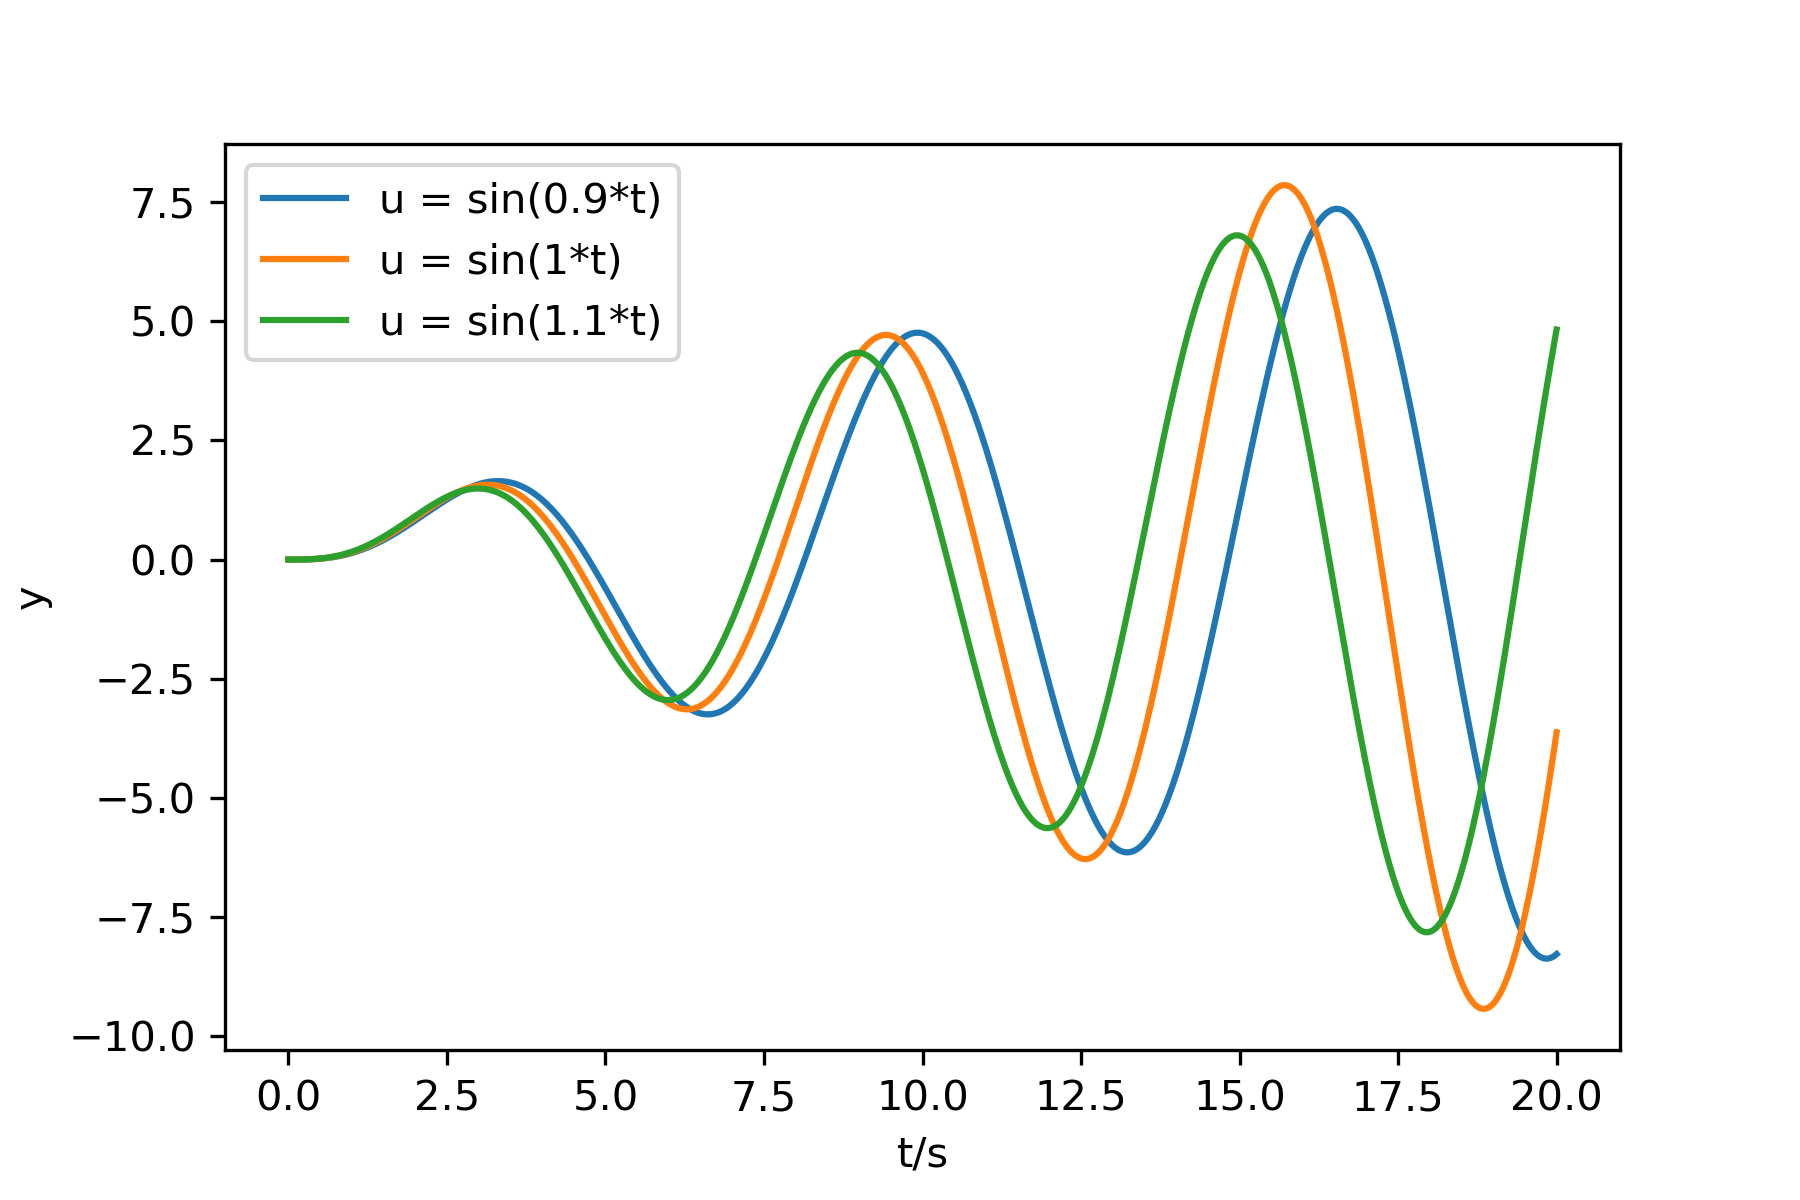
\includegraphics{figures/Resonancy.png}

    \begin{tcolorbox}[breakable, size=fbox, boxrule=1pt, pad at break*=1mm,colback=cellbackground, colframe=cellborder]
\prompt{In}{incolor}{ }{\boxspacing}
\begin{Verbatim}[commandchars=\\\{\}]

\end{Verbatim}
\end{tcolorbox}

    \hypertarget{more-realistic-model}{%
\subsection{More realistic model}\label{more-realistic-model}}

In the sequel, we consider a mass-spring-damper-system (MSD-system)
governed by the differential equation \begin{equation}
\ddot{y}(t) + \frac{d}{m}\dot{y}(t) + \frac{c}{m}y(t) = \frac{1}{m}u(t)
\end{equation} or, in state-space form, \begin{equation}
\mathbf{A} = \begin{bmatrix}%{ccccc}
             0 & 1\\
            -a_{0} & -a_{1}   
            \end{bmatrix}
            = \begin{bmatrix}%{ccccc}
             0 & 1\\
            -\frac{c}{m} & -\frac{d}{m}   
            \end{bmatrix},
\end{equation}

\begin{equation}
\mathbf{B} = \begin{bmatrix} 0 \\ 1\end{bmatrix} 
\end{equation}

\begin{equation}
\mathbf{C} = \begin{bmatrix} \frac{1}{m} & 0\end{bmatrix}
\end{equation}

\begin{equation*}
D = 0
\end{equation*}

The parameters are:

\begin{itemize}
\tightlist
\item
  Mass \(m\)
\item
  Spring constant \(c\)
\item
  Damper constant \(b\)
\end{itemize}

Such a system can be defined parametrically, so we can quickly re-run
the simulation for different systems.

    \begin{tcolorbox}[breakable, size=fbox, boxrule=1pt, pad at break*=1mm,colback=cellbackground, colframe=cellborder]
\prompt{In}{incolor}{3}{\boxspacing}
\begin{Verbatim}[commandchars=\\\{\}]
\PY{c+c1}{\PYZsh{} Parameter definition}
\PY{n}{m} \PY{o}{=} \PY{l+m+mi}{10}
\PY{n}{c} \PY{o}{=} \PY{l+m+mi}{5}
\PY{n}{d} \PY{o}{=} \PY{l+m+mi}{1}
\PY{c+c1}{\PYZsh{} State space arrays}
\PY{n}{A} \PY{o}{=} \PY{n}{array}\PY{p}{(}\PY{p}{[}\PY{p}{[}\PY{l+m+mi}{0}\PY{p}{,}\PY{l+m+mi}{1}\PY{p}{]}\PY{p}{,}\PY{p}{[}\PY{o}{\PYZhy{}}\PY{n}{c}\PY{o}{/}\PY{n}{m}\PY{p}{,} \PY{o}{\PYZhy{}}\PY{n}{d}\PY{o}{/}\PY{n}{m}\PY{p}{]}\PY{p}{]}\PY{p}{)}
\PY{n}{B} \PY{o}{=} \PY{n}{array}\PY{p}{(}\PY{p}{[}\PY{p}{[}\PY{l+m+mi}{0}\PY{p}{]}\PY{p}{,}\PY{p}{[}\PY{l+m+mi}{1}\PY{p}{]}\PY{p}{]}\PY{p}{)}
\PY{n}{C} \PY{o}{=} \PY{n}{array}\PY{p}{(}\PY{p}{[}\PY{l+m+mi}{1}\PY{o}{/}\PY{n}{m}\PY{p}{,} \PY{l+m+mi}{0}\PY{p}{]}\PY{p}{)}
\PY{n}{sys} \PY{o}{=} \PY{n}{StateSpace}\PY{p}{(}\PY{n}{A}\PY{p}{,} \PY{n}{B}\PY{p}{,} \PY{n}{C}\PY{p}{,} \PY{l+m+mi}{0}\PY{p}{)}
\end{Verbatim}
\end{tcolorbox}

    \hypertarget{system-behaviour}{%
\subsection{System behaviour}\label{system-behaviour}}

Investigate system behaviour by help of a step response.

    \begin{tcolorbox}[breakable, size=fbox, boxrule=1pt, pad at break*=1mm,colback=cellbackground, colframe=cellborder]
\prompt{In}{incolor}{4}{\boxspacing}
\begin{Verbatim}[commandchars=\\\{\}]
\PY{n}{Tin} \PY{o}{=} \PY{n}{linspace}\PY{p}{(}\PY{l+m+mi}{0}\PY{p}{,}\PY{l+m+mi}{60}\PY{p}{,} \PY{l+m+mi}{1000}\PY{p}{)}
\PY{n}{T}\PY{p}{,} \PY{n}{yout} \PY{o}{=} \PY{n}{step\PYZus{}response}\PY{p}{(}\PY{n}{sys}\PY{p}{,} \PY{n}{Tin}\PY{p}{)}
\PY{n}{plot}\PY{p}{(}\PY{n}{T}\PY{p}{,}\PY{n}{yout}\PY{p}{)}
\PY{n}{xlabel}\PY{p}{(}\PY{l+s+s1}{\PYZsq{}}\PY{l+s+s1}{t/s}\PY{l+s+s1}{\PYZsq{}}\PY{p}{)}
\PY{n}{ylabel}\PY{p}{(}\PY{l+s+s1}{\PYZsq{}}\PY{l+s+s1}{y}\PY{l+s+s1}{\PYZsq{}}\PY{p}{)}
\end{Verbatim}
\end{tcolorbox}

            \begin{tcolorbox}[breakable, size=fbox, boxrule=.5pt, pad at break*=1mm, opacityfill=0]
\prompt{Out}{outcolor}{4}{\boxspacing}
\begin{Verbatim}[commandchars=\\\{\}]
Text(0, 0.5, 'y')
\end{Verbatim}
\end{tcolorbox}
        
    \begin{center}
    \adjustimage{max size={0.9\linewidth}{0.9\paperheight}}{output_10_1.png}
    \end{center}
    { \hspace*{\fill} \\}
    
    \hypertarget{system-analysis}{%
\subsubsection{System analysis}\label{system-analysis}}

For a linear system, we can investigate the system behaviour well by
inspecting

\begin{itemize}
\item
  DC gain, i.e.~what is the system amplification after settling of any
  overshoots
\item
  Poles and Zeros, i.e.~is the system stable (all poles on the left hand
  side of the complex plane) and does it oscillate (complex conjugate
  pairs of poles)
\item
  Helpful combination (termed sisotool) to determine behaviour and
  stability consisting of

  \begin{itemize}
  \tightlist
  \item
    Bode plot
  \item
    Root-locus plot (mostly for closed loop systems)
  \item
    Step responce
  \end{itemize}
\end{itemize}

    \begin{tcolorbox}[breakable, size=fbox, boxrule=1pt, pad at break*=1mm,colback=cellbackground, colframe=cellborder]
\prompt{In}{incolor}{5}{\boxspacing}
\begin{Verbatim}[commandchars=\\\{\}]
\PY{c+c1}{\PYZsh{} Print out DC gain}
\PY{n+nb}{print}\PY{p}{(}\PY{l+s+s1}{\PYZsq{}}\PY{l+s+s1}{DC gain: }\PY{l+s+s1}{\PYZsq{}} \PY{o}{+}\PY{n+nb}{str}\PY{p}{(}\PY{n}{dcgain}\PY{p}{(}\PY{n}{sys}\PY{p}{)}\PY{p}{)}\PY{p}{)}
\PY{c+c1}{\PYZsh{} Open a new figure}
\PY{n}{figure}\PY{p}{(}\PY{p}{)}
\PY{c+c1}{\PYZsh{} Plot pole zero map}
\PY{n}{pzmap}\PY{p}{(}\PY{n}{sys}\PY{p}{)}
\PY{c+c1}{\PYZsh{} Open a new figure}
\PY{n}{figure}\PY{p}{(}\PY{p}{)}
\PY{c+c1}{\PYZsh{} Plot combination figure}
\PY{n}{sisotool}\PY{p}{(}\PY{n}{sys}\PY{p}{)}
\end{Verbatim}
\end{tcolorbox}

    \begin{Verbatim}[commandchars=\\\{\}]
DC gain: 0.2
    \end{Verbatim}

    \begin{center}
    \adjustimage{max size={0.9\linewidth}{0.9\paperheight}}{output_12_1.png}
    \end{center}
    { \hspace*{\fill} \\}
    
    \begin{center}
    \adjustimage{max size={0.9\linewidth}{0.9\paperheight}}{output_12_2.png}
    \end{center}
    { \hspace*{\fill} \\}
    
    \hypertarget{exercise}{%
\subsubsection{Exercise}\label{exercise}}

Define two alternative MSD-systems with

\begin{enumerate}
\def\labelenumi{\arabic{enumi}.}
\tightlist
\item
  Both poles on the imaginary axis (marginally stable)
\item
  Both poles on the real axis (left half obviously)
\end{enumerate}

and plot the pole-zero maps of each.

    \begin{tcolorbox}[breakable, size=fbox, boxrule=1pt, pad at break*=1mm,colback=cellbackground, colframe=cellborder]
\prompt{In}{incolor}{ }{\boxspacing}
\begin{Verbatim}[commandchars=\\\{\}]

\end{Verbatim}
\end{tcolorbox}

    \hypertarget{desired-closed-loop-behaviour}{%
\subsubsection{Desired closed-loop
behaviour}\label{desired-closed-loop-behaviour}}

With a pair of poles at \(\lambda_{1/2} = a\pm b j\) a quick settling
time can be achieved.

    \begin{tcolorbox}[breakable, size=fbox, boxrule=1pt, pad at break*=1mm,colback=cellbackground, colframe=cellborder]
\prompt{In}{incolor}{6}{\boxspacing}
\begin{Verbatim}[commandchars=\\\{\}]
\PY{n}{a} \PY{o}{=} \PY{o}{\PYZhy{}}\PY{l+m+mi}{5}
\PY{n}{b} \PY{o}{=} \PY{l+m+mf}{0.1}
\PY{n}{ssg} \PY{o}{=} \PY{p}{(}\PY{n}{a}\PY{o}{*}\PY{o}{*}\PY{l+m+mi}{2}\PY{o}{+}\PY{n}{b}\PY{o}{*}\PY{o}{*}\PY{l+m+mi}{2}\PY{p}{)}\PY{o}{/}\PY{n}{c}
\PY{n}{Ad} \PY{o}{=} \PY{n}{array}\PY{p}{(}\PY{p}{[}\PY{p}{[}\PY{l+m+mi}{0}\PY{p}{,}\PY{l+m+mi}{1}\PY{p}{]}\PY{p}{,}\PY{p}{[}\PY{o}{\PYZhy{}}\PY{l+m+mi}{1}\PY{o}{*}\PY{p}{(}\PY{n}{a}\PY{o}{*}\PY{o}{*}\PY{l+m+mi}{2}\PY{o}{+}\PY{n}{b}\PY{o}{*}\PY{o}{*}\PY{l+m+mi}{2}\PY{p}{)}\PY{p}{,} \PY{o}{\PYZhy{}}\PY{l+m+mi}{1}\PY{o}{*}\PY{p}{(}\PY{o}{\PYZhy{}}\PY{l+m+mi}{2}\PY{o}{*}\PY{n}{a}\PY{p}{)}\PY{p}{]}\PY{p}{]}\PY{p}{)}
\PY{n}{Bd} \PY{o}{=} \PY{n}{array}\PY{p}{(}\PY{p}{[}\PY{p}{[}\PY{l+m+mi}{0}\PY{p}{]}\PY{p}{,}\PY{p}{[}\PY{l+m+mi}{1}\PY{p}{]}\PY{p}{]}\PY{p}{)}
\PY{n}{Cd} \PY{o}{=} \PY{n}{array}\PY{p}{(}\PY{p}{[}\PY{n}{ssg}\PY{p}{,} \PY{l+m+mi}{0}\PY{p}{]}\PY{p}{)}
\PY{n}{sysd} \PY{o}{=} \PY{n}{StateSpace}\PY{p}{(}\PY{n}{Ad}\PY{p}{,} \PY{n}{Bd}\PY{p}{,} \PY{n}{Cd}\PY{p}{,} \PY{l+m+mi}{0}\PY{p}{)}
\end{Verbatim}
\end{tcolorbox}

    \begin{tcolorbox}[breakable, size=fbox, boxrule=1pt, pad at break*=1mm,colback=cellbackground, colframe=cellborder]
\prompt{In}{incolor}{7}{\boxspacing}
\begin{Verbatim}[commandchars=\\\{\}]
\PY{n}{youtd}\PY{p}{,} \PY{n}{T} \PY{o}{=} \PY{n}{step}\PY{p}{(}\PY{n}{sysd}\PY{p}{,} \PY{n}{Tin}\PY{p}{)}
\PY{n}{plot}\PY{p}{(}\PY{n}{T}\PY{p}{,}\PY{n}{youtd}\PY{p}{,} \PY{n}{label} \PY{o}{=} \PY{l+s+s1}{\PYZsq{}}\PY{l+s+s1}{Desired}\PY{l+s+s1}{\PYZsq{}}\PY{p}{)}
\PY{n}{plot}\PY{p}{(}\PY{n}{T}\PY{p}{,} \PY{n}{yout}\PY{p}{,} \PY{n}{label} \PY{o}{=} \PY{l+s+s1}{\PYZsq{}}\PY{l+s+s1}{Actual}\PY{l+s+s1}{\PYZsq{}}\PY{p}{)}
\PY{n}{legend}\PY{p}{(}\PY{p}{)}
\PY{n}{xlabel}\PY{p}{(}\PY{l+s+s1}{\PYZsq{}}\PY{l+s+s1}{t/s}\PY{l+s+s1}{\PYZsq{}}\PY{p}{)}
\PY{n}{ylabel}\PY{p}{(}\PY{l+s+s1}{\PYZsq{}}\PY{l+s+s1}{y}\PY{l+s+s1}{\PYZsq{}}\PY{p}{)}
\PY{c+c1}{\PYZsh{}savefig(\PYZsq{}plots/DesiredvsActual.png\PYZsq{}, dpi = 600)}
\end{Verbatim}
\end{tcolorbox}

            \begin{tcolorbox}[breakable, size=fbox, boxrule=.5pt, pad at break*=1mm, opacityfill=0]
\prompt{Out}{outcolor}{7}{\boxspacing}
\begin{Verbatim}[commandchars=\\\{\}]
Text(0, 0.5, 'y')
\end{Verbatim}
\end{tcolorbox}
        
    \begin{center}
    \adjustimage{max size={0.9\linewidth}{0.9\paperheight}}{output_17_1.png}
    \end{center}
    { \hspace*{\fill} \\}
    
    \hypertarget{state-feedback}{%
\subsection{State feedback}\label{state-feedback}}

Here we introduce full state feedback according to \begin{equation*}
\mathbf{F} = \begin{bmatrix} \left(a^2+b^2 - \frac{c}{m}\right) & \left(-2a - \frac{b}{m}\right)\end{bmatrix}
\end{equation*} and simulate a step response.

    \begin{tcolorbox}[breakable, size=fbox, boxrule=1pt, pad at break*=1mm,colback=cellbackground, colframe=cellborder]
\prompt{In}{incolor}{8}{\boxspacing}
\begin{Verbatim}[commandchars=\\\{\}]
\PY{n}{F} \PY{o}{=} \PY{n}{array}\PY{p}{(}\PY{p}{[}\PY{n}{a}\PY{o}{*}\PY{o}{*}\PY{l+m+mi}{2}\PY{o}{+}\PY{n}{b}\PY{o}{*}\PY{o}{*}\PY{l+m+mi}{2}\PY{o}{\PYZhy{}}\PY{n}{c}\PY{o}{/}\PY{n}{m}\PY{p}{,} \PY{o}{\PYZhy{}}\PY{l+m+mi}{2}\PY{o}{*}\PY{n}{a}\PY{o}{\PYZhy{}}\PY{n}{d}\PY{o}{/}\PY{n}{m}\PY{p}{]}\PY{p}{)}
\PY{n}{Acl} \PY{o}{=} \PY{n}{A}\PY{o}{\PYZhy{}}\PY{n}{B}\PY{o}{*}\PY{n}{F}
\PY{n}{Bcl} \PY{o}{=} \PY{n}{array}\PY{p}{(}\PY{p}{[}\PY{p}{[}\PY{l+m+mi}{0}\PY{p}{]}\PY{p}{,}\PY{p}{[}\PY{l+m+mi}{1}\PY{p}{]}\PY{p}{]}\PY{p}{)}
\PY{n}{Ccl} \PY{o}{=} \PY{n}{array}\PY{p}{(}\PY{p}{[}\PY{n}{ssg}\PY{p}{,} \PY{l+m+mi}{0}\PY{p}{]}\PY{p}{)}
\PY{n}{syscl} \PY{o}{=} \PY{n}{StateSpace}\PY{p}{(}\PY{n}{Acl}\PY{p}{,} \PY{n}{Bcl}\PY{p}{,} \PY{n}{Ccl}\PY{p}{,}\PY{l+m+mi}{0}\PY{p}{)}
\PY{n}{youtcl}\PY{p}{,} \PY{n}{T} \PY{o}{=} \PY{n}{step}\PY{p}{(}\PY{n}{syscl}\PY{p}{,} \PY{n}{Tin}\PY{p}{)}
\PY{n}{plot}\PY{p}{(}\PY{n}{T}\PY{p}{,}\PY{n}{youtd}\PY{p}{,} \PY{n}{label} \PY{o}{=} \PY{l+s+s1}{\PYZsq{}}\PY{l+s+s1}{Desired}\PY{l+s+s1}{\PYZsq{}}\PY{p}{,} \PY{n}{alpha} \PY{o}{=} \PY{l+m+mf}{0.7}\PY{p}{)}
\PY{n}{plot}\PY{p}{(}\PY{n}{T}\PY{p}{,} \PY{n}{yout}\PY{p}{,} \PY{n}{label} \PY{o}{=} \PY{l+s+s1}{\PYZsq{}}\PY{l+s+s1}{Actual}\PY{l+s+s1}{\PYZsq{}}\PY{p}{,} \PY{n}{alpha} \PY{o}{=} \PY{l+m+mf}{0.7}\PY{p}{)}
\PY{n}{plot}\PY{p}{(}\PY{n}{T}\PY{p}{,} \PY{n}{youtcl}\PY{p}{,} \PY{n}{label} \PY{o}{=} \PY{l+s+s1}{\PYZsq{}}\PY{l+s+s1}{Closed Loop}\PY{l+s+s1}{\PYZsq{}}\PY{p}{)}
\PY{n}{legend}\PY{p}{(}\PY{p}{)}
\PY{n}{xlabel}\PY{p}{(}\PY{l+s+s1}{\PYZsq{}}\PY{l+s+s1}{t/s}\PY{l+s+s1}{\PYZsq{}}\PY{p}{)}
\PY{n}{ylabel}\PY{p}{(}\PY{l+s+s1}{\PYZsq{}}\PY{l+s+s1}{y}\PY{l+s+s1}{\PYZsq{}}\PY{p}{)}
\PY{c+c1}{\PYZsh{}savefig(\PYZsq{}plots/DesiredvsActualvsClosedLoop.png\PYZsq{}, dpi = 600)}
\end{Verbatim}
\end{tcolorbox}

            \begin{tcolorbox}[breakable, size=fbox, boxrule=.5pt, pad at break*=1mm, opacityfill=0]
\prompt{Out}{outcolor}{8}{\boxspacing}
\begin{Verbatim}[commandchars=\\\{\}]
Text(0, 0.5, 'y')
\end{Verbatim}
\end{tcolorbox}
        
    \begin{center}
    \adjustimage{max size={0.9\linewidth}{0.9\paperheight}}{output_19_1.png}
    \end{center}
    { \hspace*{\fill} \\}
    
    \hypertarget{exercise}{%
\subsection{Exercise}\label{exercise}}

State feedback assumes perfect knowledge of the plant parameters.
Manipulate the parameters (A, B, C) of the system unknown to the
controller, check and document the results.

    \begin{tcolorbox}[breakable, size=fbox, boxrule=1pt, pad at break*=1mm,colback=cellbackground, colframe=cellborder]
\prompt{In}{incolor}{ }{\boxspacing}
\begin{Verbatim}[commandchars=\\\{\}]

\end{Verbatim}
\end{tcolorbox}

    \hypertarget{interconnections-and-feedback}{%
\subsection{Interconnections and
Feedback}\label{interconnections-and-feedback}}

It is possible to assemble dynamical systems from blocks of subsystems
by interconnection in the direction of signal flow as well as feedback.

\hypertarget{series-interconnection}{%
\subsubsection{Series interconnection}\label{series-interconnection}}

We will initially couple two first order systems:

\begin{itemize}
\tightlist
\item
  \(G_1(s) = \frac{1}{s+1}\)
\item
  \(G_2(s) = \frac{1}{s+2}\)
\end{itemize}

\begin{figure}
\centering
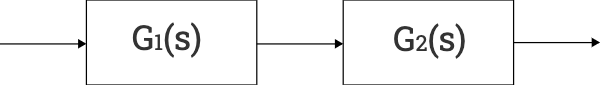
\includegraphics{figures/Interconnection.png}
\caption{System interconnection}
\end{figure}

The resulting System, \(G(s) = G_1(s) G_2(s)\), is then subjected to a
step response and compared to the individual subsystems. In the
resulting plot, we clearly see the second order nature of the
interconnected response.

    \begin{tcolorbox}[breakable, size=fbox, boxrule=1pt, pad at break*=1mm,colback=cellbackground, colframe=cellborder]
\prompt{In}{incolor}{9}{\boxspacing}
\begin{Verbatim}[commandchars=\\\{\}]
\PY{c+c1}{\PYZsh{} Create both system}
\PY{n}{sys1} \PY{o}{=} \PY{n}{tf}\PY{p}{(}\PY{p}{[}\PY{l+m+mi}{1}\PY{p}{]}\PY{p}{,}\PY{p}{[}\PY{l+m+mi}{1}\PY{p}{,} \PY{l+m+mi}{1}\PY{p}{]}\PY{p}{)}
\PY{n}{sys2} \PY{o}{=} \PY{n}{tf}\PY{p}{(}\PY{p}{[}\PY{l+m+mi}{1}\PY{p}{]}\PY{p}{,}\PY{p}{[}\PY{l+m+mi}{1}\PY{p}{,} \PY{l+m+mi}{2}\PY{p}{]}\PY{p}{)}

\PY{c+c1}{\PYZsh{} Series interconnection}
\PY{n}{sys} \PY{o}{=} \PY{n}{series}\PY{p}{(}\PY{n}{sys1}\PY{p}{,} \PY{n}{sys2}\PY{p}{)}
\PY{c+c1}{\PYZsh{} Step response simulation}
\PY{n}{T}\PY{p}{,} \PY{n}{yout} \PY{o}{=} \PY{n}{step\PYZus{}response}\PY{p}{(}\PY{n}{sys}\PY{p}{)}
\PY{n}{T1}\PY{p}{,} \PY{n}{yout1} \PY{o}{=} \PY{n}{step\PYZus{}response}\PY{p}{(}\PY{n}{sys1}\PY{p}{)}
\PY{n}{T2}\PY{p}{,} \PY{n}{yout2} \PY{o}{=} \PY{n}{step\PYZus{}response}\PY{p}{(}\PY{n}{sys2}\PY{p}{)}
\PY{c+c1}{\PYZsh{} Plotting}
\PY{n}{plot}\PY{p}{(}\PY{n}{T}\PY{p}{,} \PY{n}{yout}\PY{p}{,} \PY{n}{label} \PY{o}{=} \PY{l+s+s1}{\PYZsq{}}\PY{l+s+s1}{G(s)}\PY{l+s+s1}{\PYZsq{}}\PY{p}{)}
\PY{n}{plot}\PY{p}{(}\PY{n}{T1}\PY{p}{,} \PY{n}{yout1}\PY{p}{,} \PY{n}{label} \PY{o}{=} \PY{l+s+s1}{\PYZsq{}}\PY{l+s+s1}{G\PYZus{}1(s)}\PY{l+s+s1}{\PYZsq{}}\PY{p}{)}
\PY{n}{plot}\PY{p}{(}\PY{n}{T2}\PY{p}{,} \PY{n}{yout2}\PY{p}{,} \PY{n}{label} \PY{o}{=} \PY{l+s+s1}{\PYZsq{}}\PY{l+s+s1}{G\PYZus{}2(s)}\PY{l+s+s1}{\PYZsq{}}\PY{p}{)}
\PY{n}{legend}\PY{p}{(}\PY{p}{)}
\PY{n}{xlabel}\PY{p}{(}\PY{l+s+s1}{\PYZsq{}}\PY{l+s+s1}{t/s}\PY{l+s+s1}{\PYZsq{}}\PY{p}{)}
\PY{n}{ylabel}\PY{p}{(}\PY{l+s+s1}{\PYZsq{}}\PY{l+s+s1}{y}\PY{l+s+s1}{\PYZsq{}}\PY{p}{)}
\end{Verbatim}
\end{tcolorbox}

            \begin{tcolorbox}[breakable, size=fbox, boxrule=.5pt, pad at break*=1mm, opacityfill=0]
\prompt{Out}{outcolor}{9}{\boxspacing}
\begin{Verbatim}[commandchars=\\\{\}]
Text(0, 0.5, 'y')
\end{Verbatim}
\end{tcolorbox}
        
    \begin{center}
    \adjustimage{max size={0.9\linewidth}{0.9\paperheight}}{output_23_1.png}
    \end{center}
    { \hspace*{\fill} \\}
    
    \hypertarget{feedback-interconnection}{%
\subsubsection{Feedback
interconnection}\label{feedback-interconnection}}

For the feedback interconnection, we will add a feedback compensator to
the heavily overshooting plant \[G_1(s) = \frac{20}{s^2+2s+20}\]
according to the transfer function \[G_{comp} = K s.\]

    \begin{tcolorbox}[breakable, size=fbox, boxrule=1pt, pad at break*=1mm,colback=cellbackground, colframe=cellborder]
\prompt{In}{incolor}{10}{\boxspacing}
\begin{Verbatim}[commandchars=\\\{\}]
\PY{c+c1}{\PYZsh{} Generate both systems}
\PY{n}{sys1} \PY{o}{=} \PY{n}{tf}\PY{p}{(}\PY{p}{[}\PY{l+m+mi}{20}\PY{p}{]}\PY{p}{,}\PY{p}{[}\PY{l+m+mi}{1}\PY{p}{,} \PY{l+m+mi}{2}\PY{p}{,} \PY{l+m+mi}{20}\PY{p}{]}\PY{p}{)}
\PY{c+c1}{\PYZsh{} Parametric gain}
\PY{n}{K} \PY{o}{=} \PY{o}{.}\PY{l+m+mi}{35}
\PY{n}{comp} \PY{o}{=} \PY{n}{tf}\PY{p}{(}\PY{p}{[}\PY{n}{K}\PY{p}{,} \PY{l+m+mi}{0}\PY{p}{]}\PY{p}{,} \PY{p}{[}\PY{l+m+mi}{1}\PY{p}{]}\PY{p}{)}

\PY{c+c1}{\PYZsh{}\PYZsh{}\PYZsh{}\PYZsh{}\PYZsh{}\PYZsh{}\PYZsh{}\PYZsh{}\PYZsh{}\PYZsh{}\PYZsh{}\PYZsh{}\PYZsh{}\PYZsh{}\PYZsh{}\PYZsh{}\PYZsh{}\PYZsh{}\PYZsh{}\PYZsh{}\PYZsh{}\PYZsh{}\PYZsh{}\PYZsh{}\PYZsh{}\PYZsh{}}
\PY{c+c1}{\PYZsh{} Feedback interconnection}
\PY{n}{sys} \PY{o}{=} \PY{n}{feedback}\PY{p}{(}\PY{n}{sys1}\PY{p}{,} \PY{n}{comp}\PY{p}{)}

\PY{c+c1}{\PYZsh{}\PYZsh{}\PYZsh{}\PYZsh{}\PYZsh{}\PYZsh{}\PYZsh{}\PYZsh{}\PYZsh{}\PYZsh{}\PYZsh{}\PYZsh{}\PYZsh{}\PYZsh{}\PYZsh{}\PYZsh{}\PYZsh{}\PYZsh{}\PYZsh{}\PYZsh{}\PYZsh{}\PYZsh{}\PYZsh{}\PYZsh{}\PYZsh{}\PYZsh{}\PYZsh{}}
\PY{c+c1}{\PYZsh{} Print the overall system}
\PY{n+nb}{print}\PY{p}{(}\PY{l+s+s1}{\PYZsq{}}\PY{l+s+s1}{G(s) = }\PY{l+s+s1}{\PYZsq{}} \PY{o}{+} \PY{n+nb}{str}\PY{p}{(}\PY{n}{sys}\PY{p}{)}\PY{p}{)}
\PY{c+c1}{\PYZsh{} Print poles of closed loop system}
\PY{n+nb}{print}\PY{p}{(}\PY{l+s+s1}{\PYZsq{}}\PY{l+s+s1}{Poles of closed loop system: }\PY{l+s+s1}{\PYZsq{}} \PY{o}{+} \PY{n+nb}{str}\PY{p}{(}\PY{n}{pole}\PY{p}{(}\PY{n}{sys}\PY{p}{)}\PY{p}{)}\PY{p}{)}

\PY{c+c1}{\PYZsh{}\PYZsh{}\PYZsh{}\PYZsh{}\PYZsh{}\PYZsh{}\PYZsh{}\PYZsh{}\PYZsh{}\PYZsh{}\PYZsh{}\PYZsh{}\PYZsh{}\PYZsh{}\PYZsh{}\PYZsh{}\PYZsh{}\PYZsh{}\PYZsh{}\PYZsh{}\PYZsh{}\PYZsh{}\PYZsh{}\PYZsh{}\PYZsh{}\PYZsh{}\PYZsh{}}
\PY{c+c1}{\PYZsh{} Plotting}
\PY{n}{T}\PY{p}{,} \PY{n}{yout} \PY{o}{=} \PY{n}{step\PYZus{}response}\PY{p}{(}\PY{n}{sys}\PY{p}{,}\PY{n}{Tin}\PY{p}{)}
\PY{n}{T1}\PY{p}{,} \PY{n}{yout1} \PY{o}{=} \PY{n}{step\PYZus{}response}\PY{p}{(}\PY{n}{sys1}\PY{p}{,} \PY{n}{Tin}\PY{p}{)}
\PY{n}{plot}\PY{p}{(}\PY{n}{T}\PY{p}{,} \PY{n}{yout}\PY{p}{,} \PY{n}{label} \PY{o}{=} \PY{l+s+s1}{\PYZsq{}}\PY{l+s+s1}{G(s)}\PY{l+s+s1}{\PYZsq{}}\PY{p}{)}
\PY{n}{plot}\PY{p}{(}\PY{n}{T1}\PY{p}{,} \PY{n}{yout1}\PY{p}{,} \PY{n}{label} \PY{o}{=} \PY{l+s+s1}{\PYZsq{}}\PY{l+s+s1}{G\PYZus{}1(s)}\PY{l+s+s1}{\PYZsq{}}\PY{p}{)}
\PY{n}{legend}\PY{p}{(}\PY{p}{)}
\PY{n}{grid}\PY{p}{(}\PY{p}{)}
\PY{n}{xlabel}\PY{p}{(}\PY{l+s+s1}{\PYZsq{}}\PY{l+s+s1}{t/s}\PY{l+s+s1}{\PYZsq{}}\PY{p}{)}
\PY{n}{ylabel}\PY{p}{(}\PY{l+s+s1}{\PYZsq{}}\PY{l+s+s1}{y}\PY{l+s+s1}{\PYZsq{}}\PY{p}{)}
\end{Verbatim}
\end{tcolorbox}

    \begin{Verbatim}[commandchars=\\\{\}]
G(s) =
      20
--------------
s\^{}2 + 9 s + 20

Poles of closed loop system: [-5. -4.]
    \end{Verbatim}

            \begin{tcolorbox}[breakable, size=fbox, boxrule=.5pt, pad at break*=1mm, opacityfill=0]
\prompt{Out}{outcolor}{10}{\boxspacing}
\begin{Verbatim}[commandchars=\\\{\}]
Text(0, 0.5, 'y')
\end{Verbatim}
\end{tcolorbox}
        
    \begin{center}
    \adjustimage{max size={0.9\linewidth}{0.9\paperheight}}{output_25_2.png}
    \end{center}
    { \hspace*{\fill} \\}
    
    \hypertarget{dc-motor-example}{%
\subsection{DC Motor example}\label{dc-motor-example}}

A linear model of a DC motor consists of a mechanical part and the
electrical part.

The mechanical part is a rotating mass, so exhibiting inertia \(J\) as
well as some damping \(B\).

The electrical subsystem consists of the armature resistance \(R_a\),
the armature inductance \(L_a\). A loop according to Kirchhoff's Law
also reveals a back-EMF voltage \(U_b\).

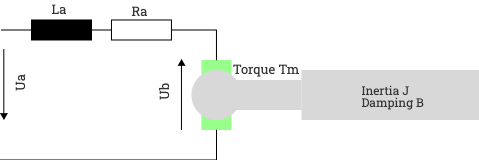
\includegraphics{figures/DCMotor.png}

This back-EMF is linked to the rotational velocity \(\omega\) according
to \[U_b = K_b \omega\] while the generated torque is depending on the
current in the armature \(I_a\) according to \[T = K_T I_a.\]

The input voltage \(U_a\) drives the armature current according to
\[U_a = L_a \frac{dI_a}{dt} + R_a I_a + U_b,\] after a Laplace Transform
yielding the transfer function
\[\frac{I_a}{U_a - U_b} = \frac{1}{L_a s+R_a}\] for the electrical
subsystem. Note the transfer of \[U_a - U_b \rightarrow I_a,\]
indicating a feedback from the output velocity.

The mechanical subsystem is an inertial, damped system, governed by the
transfer function \[\frac{\omega}{T_m} = \frac{1}{Js+B}\].

The back-EMF is proportional to \(\omega\) according to
\[Ub = K_b \omega.\]

The overall block diagram is shown below:

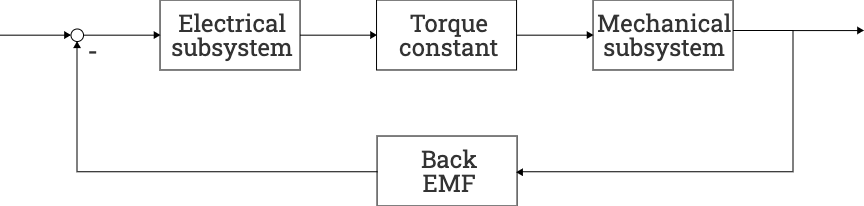
\includegraphics{figures/DCMotorBlock.png}

    \hypertarget{exercise}{%
\subsection{Exercise}\label{exercise}}

Implement a DC motor model and simulate the step response as well as a
forced response to a sinewave.

\begin{enumerate}
\def\labelenumi{\arabic{enumi}.}
\tightlist
\item
  Define the system parameters:

  \begin{itemize}
  \tightlist
  \item
    \(R_a = 5\)
  \item
    \(L_a = 0.1\)
  \item
    \(K_T = 10\)
  \item
    \(J = 1\)
  \item
    \(B = 0.001\)
  \item
    \(K_b = 1\)
  \end{itemize}
\item
  Model the subsystems:

  \begin{enumerate}
  \def\labelenumii{\arabic{enumii}.}
  \tightlist
  \item
    Electrical subsystem
  \item
    Torque constant \(K_T\) as a transfer function
    \texttt{tf({[}KT{]},{[}1{]})}
  \item
    Mechanical subsystem
  \item
    Back-EMF constant as \(K_T\)
  \end{enumerate}
\item
  Interconnect according to the block diagram above

  \begin{enumerate}
  \def\labelenumii{\arabic{enumii}.}
  \tightlist
  \item
    Start with forward path
  \item
    Add feedback
  \end{enumerate}
\item
  Simulate and plot

  \begin{enumerate}
  \def\labelenumii{\arabic{enumii}.}
  \tightlist
  \item
    subject the system to a unit step
  \item
    Subject the system to a 12V-sine voltage with \(2\pi\) frequency.
    Use the code snippets
  \end{enumerate}

\begin{Shaded}
\begin{Highlighting}[]
\NormalTok{figure(figsize}\OperatorTok{=}\NormalTok{(}\DecValTok{10}\NormalTok{,}\DecValTok{6}\NormalTok{))}
\NormalTok{subplot(}\DecValTok{3}\NormalTok{,}\DecValTok{1}\NormalTok{,(}\DecValTok{1}\NormalTok{,}\DecValTok{2}\NormalTok{))}
\end{Highlighting}
\end{Shaded}

  and \textasciitilde{}\sout{.py figure(figsize=(10,6))
  subplot(3,1,3)}\textasciitilde{} to replicate this figure:
  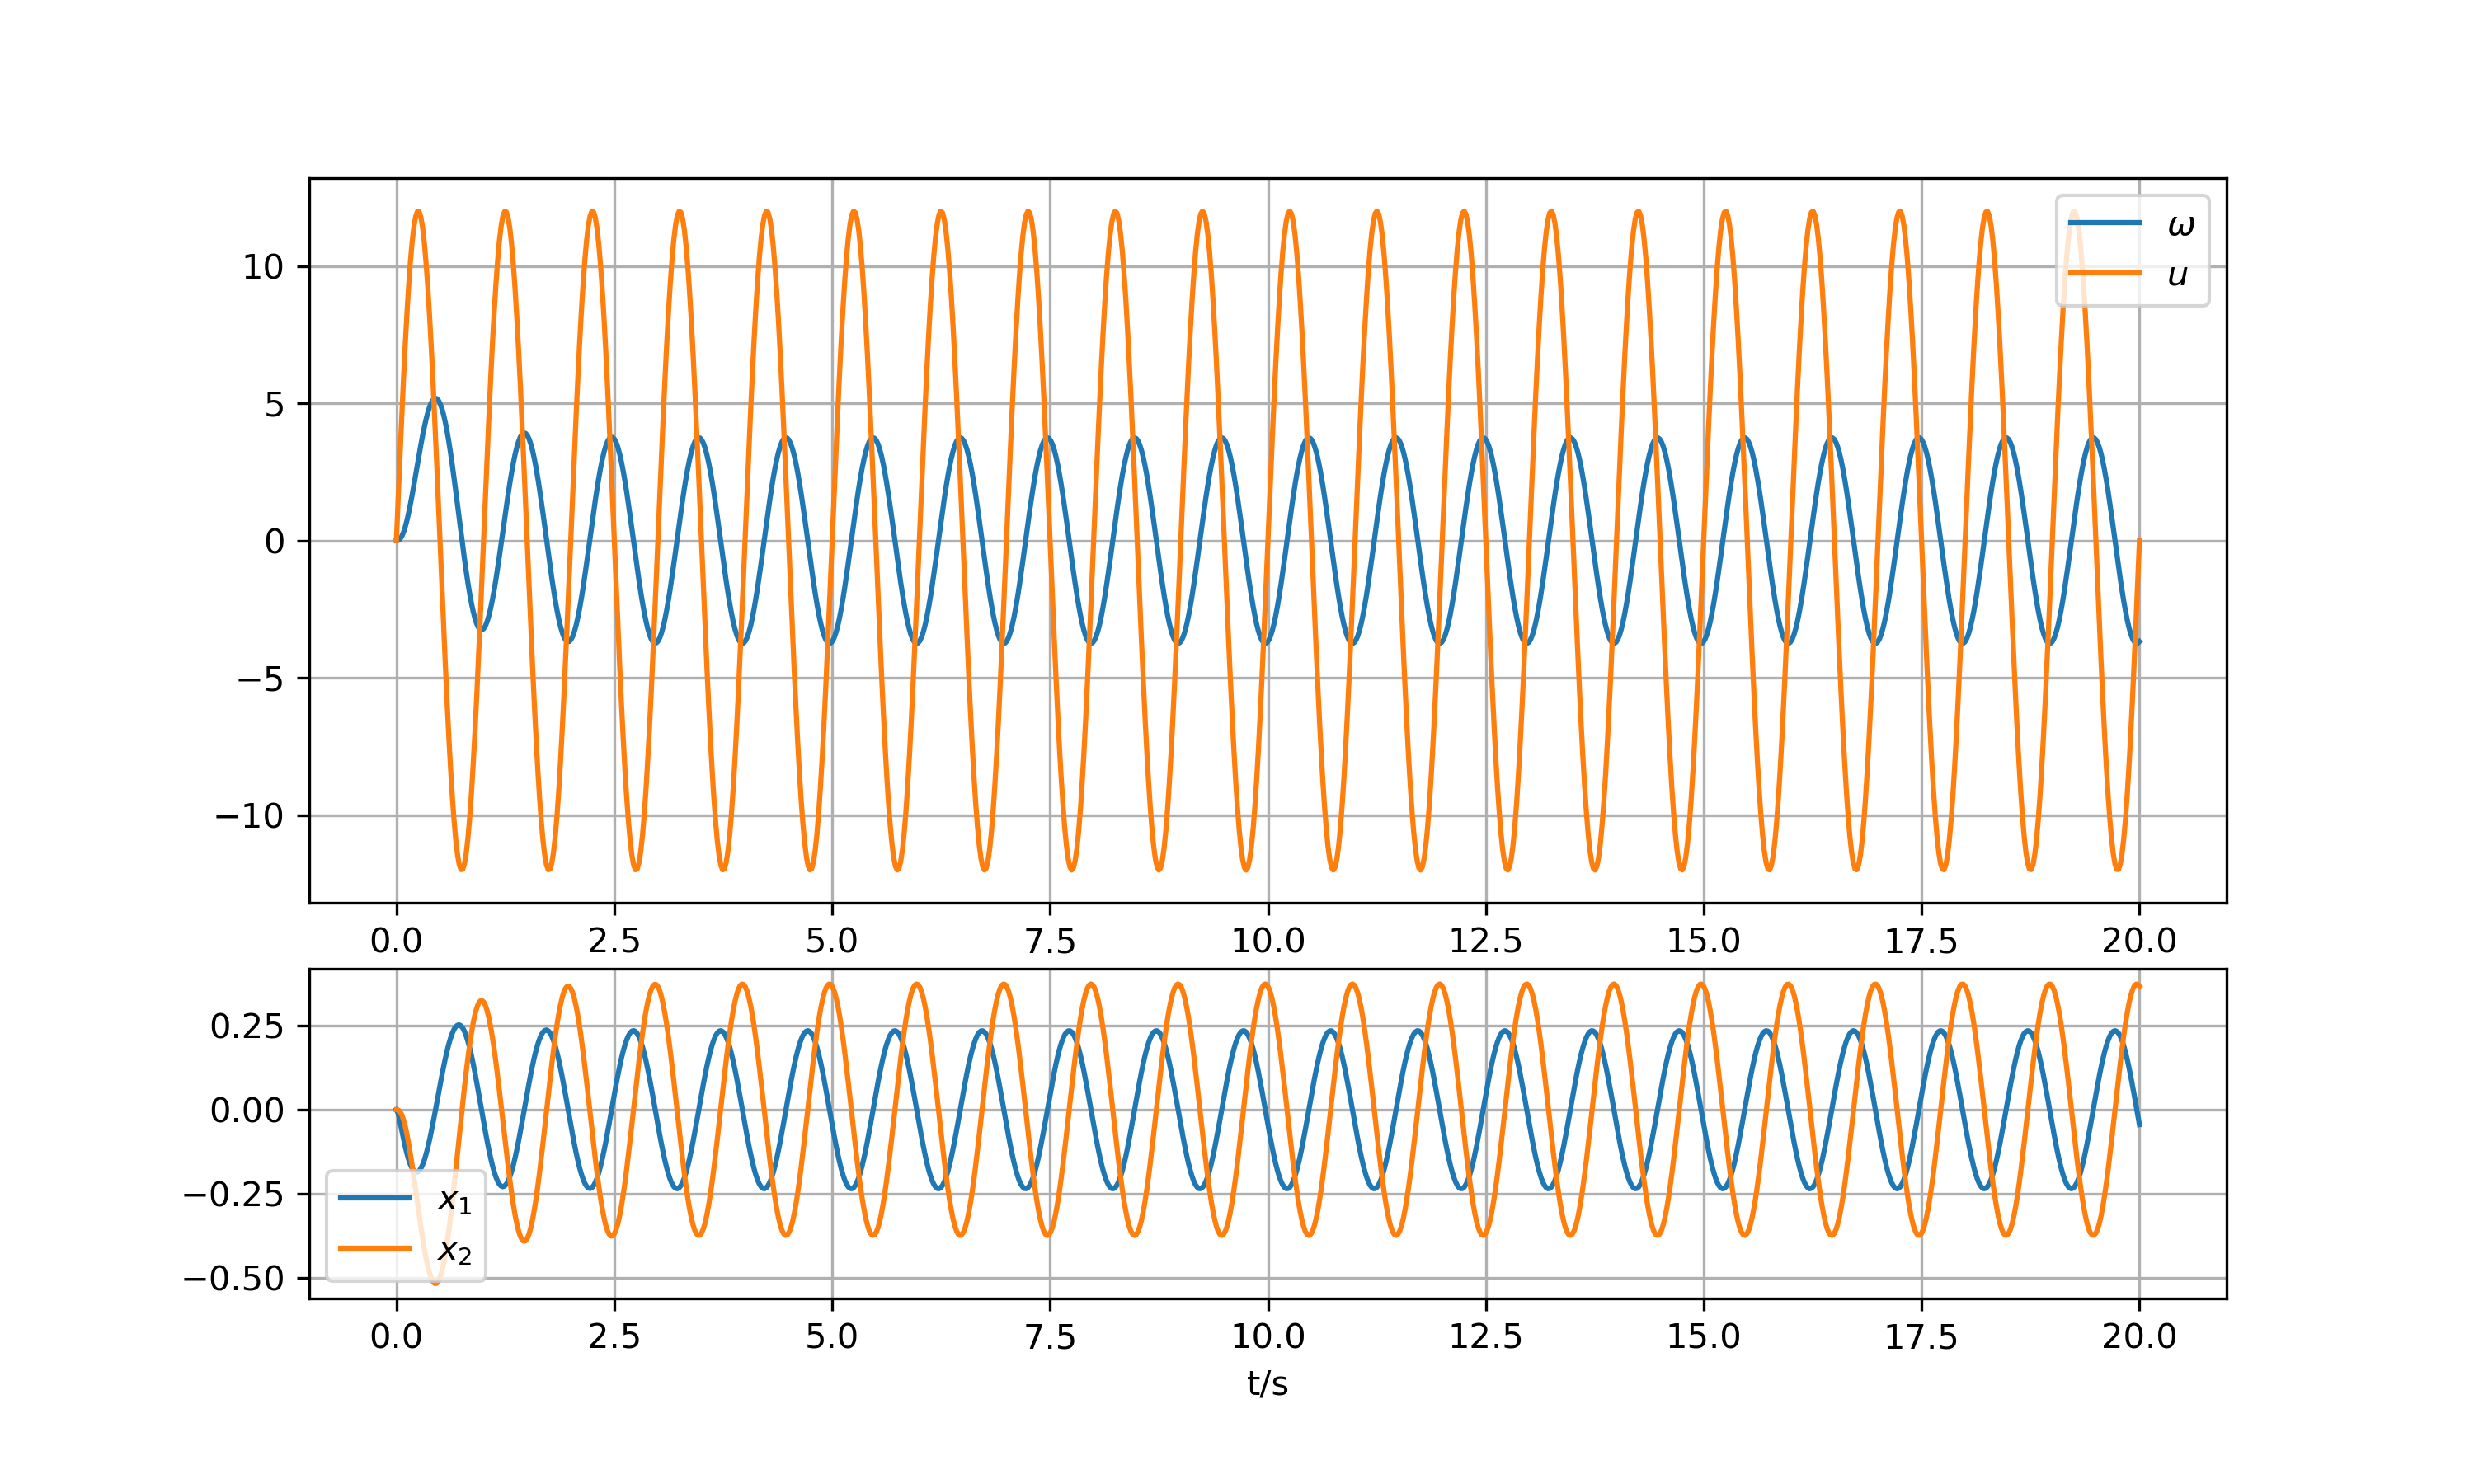
\includegraphics{figures/DCMotorSim.png}
\end{enumerate}

    \begin{tcolorbox}[breakable, size=fbox, boxrule=1pt, pad at break*=1mm,colback=cellbackground, colframe=cellborder]
\prompt{In}{incolor}{ }{\boxspacing}
\begin{Verbatim}[commandchars=\\\{\}]

\end{Verbatim}
\end{tcolorbox}

    \hypertarget{nonlinear-systems}{%
\subsection{Nonlinear systems}\label{nonlinear-systems}}

As a nonlinear system example, we consider the mathematical pendulum as
depicted below:

\begin{figure}
\centering
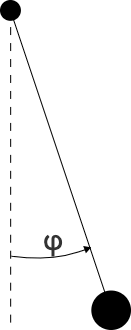
\includegraphics{figures/Pendulum.png}
\caption{Pendulum}
\end{figure}

This system is governed by the differential equation
\[\ddot{\varphi} + \frac{g}{l}\sin(\varphi) = 0\]

While linear systems are somewhat easier to handle, we need to
explicitly define the function to transfer the states. Also we need to
import and utilise an ODE solver, which is contained in the
scipy.integrate library.

    \begin{tcolorbox}[breakable, size=fbox, boxrule=1pt, pad at break*=1mm,colback=cellbackground, colframe=cellborder]
\prompt{In}{incolor}{14}{\boxspacing}
\begin{Verbatim}[commandchars=\\\{\}]
\PY{k+kn}{from} \PY{n+nn}{scipy} \PY{k+kn}{import} \PY{n}{integrate}
\end{Verbatim}
\end{tcolorbox}

    Next, we need to define the nonlinear differential equation in terms of
a first order differential equation, i.e.~mapping a state vector \(x\)
to its derivative \(\dot{x} = f(x)\). Since time dependence can be
implemented, it needs to accept both time and state.

The state space representation of the above ODE is

\[\dot{x} = \begin{pmatrix} \dot{x}_1 \\ \dot{x}_2 \end{pmatrix}  = \begin{pmatrix} x_2 \\ \frac{-g}{l}\sin\left(x_2\right) \end{pmatrix}.\]

This is implemented below:

    \begin{tcolorbox}[breakable, size=fbox, boxrule=1pt, pad at break*=1mm,colback=cellbackground, colframe=cellborder]
\prompt{In}{incolor}{11}{\boxspacing}
\begin{Verbatim}[commandchars=\\\{\}]
\PY{c+c1}{\PYZsh{}\PYZsh{} Nonlinear state space function}
\PY{k}{def} \PY{n+nf}{f}\PY{p}{(}\PY{n}{x}\PY{p}{,}\PY{n}{t}\PY{o}{=}\PY{l+m+mi}{0}\PY{p}{)}\PY{p}{:}
    \PY{c+c1}{\PYZsh{} Parameters}
    \PY{n}{g} \PY{o}{=} \PY{l+m+mf}{9.81}
    \PY{n}{l} \PY{o}{=} \PY{l+m+mi}{10}
    \PY{c+c1}{\PYZsh{} Return state differential}
    \PY{k}{return} \PY{p}{[}\PY{n}{x}\PY{p}{[}\PY{l+m+mi}{1}\PY{p}{]}\PY{p}{,} \PY{o}{\PYZhy{}}\PY{n}{g}\PY{o}{/}\PY{n}{l}\PY{o}{*}\PY{n}{np}\PY{o}{.}\PY{n}{sin}\PY{p}{(}\PY{n}{x}\PY{p}{[}\PY{l+m+mi}{0}\PY{p}{]}\PY{p}{)}\PY{p}{]}
\end{Verbatim}
\end{tcolorbox}

    \hypertarget{phase-portrait}{%
\subsubsection{Phase portrait}\label{phase-portrait}}

A good way to think about nonlinear systems is to consider their phase
portrait, i.e.~a directional field to observer their evolution from an
arbitrary starting point.

For this purpose, we use \texttt{meshgrid} to generate linear increasing
matrices over a given value range.

    \begin{tcolorbox}[breakable, size=fbox, boxrule=1pt, pad at break*=1mm,colback=cellbackground, colframe=cellborder]
\prompt{In}{incolor}{15}{\boxspacing}
\begin{Verbatim}[commandchars=\\\{\}]
\PY{c+c1}{\PYZsh{} Create figure and axis objects}
\PY{n}{fig} \PY{o}{=} \PY{n}{figure}\PY{p}{(}\PY{n}{num}\PY{o}{=}\PY{l+m+mi}{1}\PY{p}{,} \PY{n}{figsize} \PY{o}{=} \PY{p}{(}\PY{l+m+mi}{12}\PY{p}{,}\PY{l+m+mi}{5}\PY{p}{)}\PY{p}{)}
\PY{n}{ax}\PY{o}{=}\PY{n}{fig}\PY{o}{.}\PY{n}{add\PYZus{}subplot}\PY{p}{(}\PY{l+m+mi}{111}\PY{p}{)}
\PY{c+c1}{\PYZsh{} Create two matrices}
\PY{n}{X1}\PY{p}{,}\PY{n}{X2} \PY{o}{=} \PY{n}{np}\PY{o}{.}\PY{n}{meshgrid}\PY{p}{(}\PY{n}{np}\PY{o}{.}\PY{n}{linspace}\PY{p}{(}\PY{o}{\PYZhy{}}\PY{l+m+mi}{2}\PY{o}{*}\PY{n}{np}\PY{o}{.}\PY{n}{pi}\PY{p}{,}\PY{l+m+mi}{2}\PY{o}{*}\PY{n}{np}\PY{o}{.}\PY{n}{pi}\PY{p}{,}\PY{l+m+mi}{40}\PY{p}{)}\PY{p}{,}\PY{n}{np}\PY{o}{.}\PY{n}{linspace}\PY{p}{(}\PY{o}{\PYZhy{}}\PY{n}{np}\PY{o}{.}\PY{n}{pi}\PY{o}{/}\PY{l+m+mi}{2}\PY{p}{,}\PY{n}{np}\PY{o}{.}\PY{n}{pi}\PY{o}{/}\PY{l+m+mi}{2}\PY{p}{,}\PY{l+m+mi}{10}\PY{p}{)}\PY{p}{)}
\PY{c+c1}{\PYZsh{} Calculate differentials}
\PY{n}{DX1}\PY{p}{,} \PY{n}{DX2} \PY{o}{=} \PY{n}{f}\PY{p}{(}\PY{p}{[}\PY{n}{X1}\PY{p}{,}\PY{n}{X2}\PY{p}{]}\PY{p}{)}
\PY{c+c1}{\PYZsh{} Plot as a vector field}
\PY{n}{ax}\PY{o}{.}\PY{n}{quiver}\PY{p}{(}\PY{n}{X1}\PY{p}{,}\PY{n}{X2}\PY{p}{,}\PY{n}{DX1}\PY{p}{,}\PY{n}{DX2}\PY{p}{)}
\PY{c+c1}{\PYZsh{} Label axes}
\PY{n}{xlabel}\PY{p}{(}\PY{l+s+s2}{\PYZdq{}}\PY{l+s+s2}{\PYZdl{}x\PYZus{}1\PYZdl{}}\PY{l+s+s2}{\PYZdq{}}\PY{p}{)}
\PY{n}{ylabel}\PY{p}{(}\PY{l+s+s2}{\PYZdq{}}\PY{l+s+s2}{\PYZdl{}x\PYZus{}2\PYZdl{}}\PY{l+s+s2}{\PYZdq{}}\PY{p}{)}
\end{Verbatim}
\end{tcolorbox}

            \begin{tcolorbox}[breakable, size=fbox, boxrule=.5pt, pad at break*=1mm, opacityfill=0]
\prompt{Out}{outcolor}{15}{\boxspacing}
\begin{Verbatim}[commandchars=\\\{\}]
Text(0, 0.5, '\$x\_2\$')
\end{Verbatim}
\end{tcolorbox}
        
    \begin{center}
    \adjustimage{max size={0.9\linewidth}{0.9\paperheight}}{output_34_1.png}
    \end{center}
    { \hspace*{\fill} \\}
    
    In the phase portrait, we clearly see the points of stability for
\((k\pi,0)^T,\, k = 0, 1,\ldots\), with even \(k\) indicating the lower
point of stability.

It is time to plot some trajectories. To achieve this, we solve the ODE
using \texttt{integrate.odeint} with options:

\begin{itemize}
\tightlist
\item
  f, the name of the function
\item
  x0, the initial state
\item
  t, a time vector defined beforehand
\end{itemize}

The return value is an array of the state evolution, which can be
plotted after transposing. In order to evaluate the different initial
conditions, we loop through these.

    \begin{tcolorbox}[breakable, size=fbox, boxrule=1pt, pad at break*=1mm,colback=cellbackground, colframe=cellborder]
\prompt{In}{incolor}{16}{\boxspacing}
\begin{Verbatim}[commandchars=\\\{\}]
\PY{n}{fig} \PY{o}{=} \PY{n}{figure}\PY{p}{(}\PY{n}{num}\PY{o}{=}\PY{l+m+mi}{1}\PY{p}{,} \PY{n}{figsize} \PY{o}{=} \PY{p}{(}\PY{l+m+mi}{12}\PY{p}{,}\PY{l+m+mi}{5}\PY{p}{)}\PY{p}{)}
\PY{n}{ax}\PY{o}{=}\PY{n}{fig}\PY{o}{.}\PY{n}{add\PYZus{}subplot}\PY{p}{(}\PY{l+m+mi}{111}\PY{p}{)}
\PY{c+c1}{\PYZsh{} Time axis for solution (with fine resolution)}
\PY{n}{t} \PY{o}{=} \PY{n}{np}\PY{o}{.}\PY{n}{linspace}\PY{p}{(}\PY{l+m+mi}{0}\PY{p}{,}\PY{l+m+mi}{50}\PY{p}{,}\PY{l+m+mi}{1000}\PY{p}{)}
\PY{c+c1}{\PYZsh{} Array of initial conditions}
\PY{n}{X0} \PY{o}{=} \PY{p}{[}\PY{n}{np}\PY{o}{.}\PY{n}{array}\PY{p}{(}\PY{p}{[}\PY{l+m+mi}{1}\PY{p}{,}\PY{l+m+mi}{0}\PY{p}{]}\PY{p}{)}\PY{p}{,} \PY{n}{np}\PY{o}{.}\PY{n}{array}\PY{p}{(}\PY{p}{[}\PY{o}{\PYZhy{}}\PY{l+m+mi}{10}\PY{p}{,}\PY{l+m+mi}{1}\PY{p}{]}\PY{p}{)}\PY{p}{,} \PY{n}{np}\PY{o}{.}\PY{n}{array}\PY{p}{(}\PY{p}{[}\PY{l+m+mf}{3.2}\PY{p}{,}\PY{l+m+mi}{0}\PY{p}{]}\PY{p}{)}\PY{p}{,} \PY{n}{np}\PY{o}{.}\PY{n}{array}\PY{p}{(}\PY{p}{[}\PY{l+m+mf}{3.1}\PY{p}{,}\PY{l+m+mi}{0}\PY{p}{]}\PY{p}{)}\PY{p}{]}

\PY{c+c1}{\PYZsh{} Plot phase portrait as above}
\PY{n}{X1}\PY{p}{,}\PY{n}{X2} \PY{o}{=} \PY{n}{np}\PY{o}{.}\PY{n}{meshgrid}\PY{p}{(}\PY{n}{np}\PY{o}{.}\PY{n}{linspace}\PY{p}{(}\PY{o}{\PYZhy{}}\PY{l+m+mi}{4}\PY{o}{*}\PY{n}{np}\PY{o}{.}\PY{n}{pi}\PY{p}{,}\PY{l+m+mi}{4}\PY{o}{*}\PY{n}{np}\PY{o}{.}\PY{n}{pi}\PY{p}{,}\PY{l+m+mi}{40}\PY{p}{)}\PY{p}{,}\PY{n}{np}\PY{o}{.}\PY{n}{linspace}\PY{p}{(}\PY{o}{\PYZhy{}}\PY{n}{np}\PY{o}{.}\PY{n}{pi}\PY{o}{/}\PY{l+m+mi}{2}\PY{p}{,}\PY{n}{np}\PY{o}{.}\PY{n}{pi}\PY{o}{/}\PY{l+m+mi}{2}\PY{p}{,}\PY{l+m+mi}{10}\PY{p}{)}\PY{p}{)}
\PY{n}{DX1}\PY{p}{,} \PY{n}{DX2} \PY{o}{=} \PY{n}{f}\PY{p}{(}\PY{p}{[}\PY{n}{X1}\PY{p}{,}\PY{n}{X2}\PY{p}{]}\PY{p}{)}
\PY{n}{ax}\PY{o}{.}\PY{n}{quiver}\PY{p}{(}\PY{n}{X1}\PY{p}{,}\PY{n}{X2}\PY{p}{,}\PY{n}{DX1}\PY{p}{,}\PY{n}{DX2}\PY{p}{)}
\PY{k}{for} \PY{n}{x0} \PY{o+ow}{in} \PY{n}{X0}\PY{p}{:}
    \PY{c+c1}{\PYZsh{} Call ODE solver}
    \PY{n}{P} \PY{o}{=} \PY{n}{integrate}\PY{o}{.}\PY{n}{odeint}\PY{p}{(}\PY{n}{f}\PY{p}{,} \PY{n}{x0}\PY{p}{,} \PY{n}{t}\PY{p}{)}\PY{o}{.}\PY{n}{T}
    \PY{c+c1}{\PYZsh{} Plot the resulting curve and add label}
    \PY{n}{ax}\PY{o}{.}\PY{n}{plot}\PY{p}{(}\PY{n}{P}\PY{p}{[}\PY{l+m+mi}{0}\PY{p}{]}\PY{p}{,}\PY{n}{P}\PY{p}{[}\PY{l+m+mi}{1}\PY{p}{]}\PY{p}{,} \PY{n}{label} \PY{o}{=} \PY{l+s+s1}{\PYZsq{}}\PY{l+s+s1}{\PYZdl{}x\PYZus{}0\PYZdl{}=}\PY{l+s+s1}{\PYZsq{}}\PY{o}{+}\PY{n+nb}{str}\PY{p}{(}\PY{n}{x0}\PY{p}{)}\PY{p}{)}
\PY{c+c1}{\PYZsh{} Limit x\PYZhy{}axis \PYZhy{} Some solutions evolve too far.}
\PY{n}{xlim}\PY{p}{(}\PY{p}{[}\PY{o}{\PYZhy{}}\PY{l+m+mi}{4}\PY{o}{*}\PY{n}{np}\PY{o}{.}\PY{n}{pi}\PY{p}{,} \PY{l+m+mi}{4}\PY{o}{*}\PY{n}{np}\PY{o}{.}\PY{n}{pi}\PY{p}{]}\PY{p}{)}
\PY{n}{xlabel}\PY{p}{(}\PY{l+s+s2}{\PYZdq{}}\PY{l+s+s2}{\PYZdl{}x\PYZus{}1\PYZdl{}}\PY{l+s+s2}{\PYZdq{}}\PY{p}{)}
\PY{n}{ylabel}\PY{p}{(}\PY{l+s+s2}{\PYZdq{}}\PY{l+s+s2}{\PYZdl{}x\PYZus{}2\PYZdl{}}\PY{l+s+s2}{\PYZdq{}}\PY{p}{)}
\PY{c+c1}{\PYZsh{} Show initial condition labels}
\PY{n}{legend}\PY{p}{(}\PY{p}{)}
\end{Verbatim}
\end{tcolorbox}

            \begin{tcolorbox}[breakable, size=fbox, boxrule=.5pt, pad at break*=1mm, opacityfill=0]
\prompt{Out}{outcolor}{16}{\boxspacing}
\begin{Verbatim}[commandchars=\\\{\}]
<matplotlib.legend.Legend at 0x15dd605b0>
\end{Verbatim}
\end{tcolorbox}
        
    \begin{center}
    \adjustimage{max size={0.9\linewidth}{0.9\paperheight}}{output_36_1.png}
    \end{center}
    { \hspace*{\fill} \\}
    
    \hypertarget{exercise}{%
\subsection{Exercise}\label{exercise}}

Extend the nonlinear system example above to include friction, the
updated state space formulation shall be

\[\dot{x} = \begin{pmatrix} \dot{x}_1 \\ \dot{x}_2 \end{pmatrix}  = \begin{pmatrix} x_2  \\ \frac{-g}{l}\sin\left(x_2\right) - \mu x_1 \end{pmatrix}.\]

Select \(\mu = 0.1\) as a friction coefficient and plot the according
trajectories.

    \begin{tcolorbox}[breakable, size=fbox, boxrule=1pt, pad at break*=1mm,colback=cellbackground, colframe=cellborder]
\prompt{In}{incolor}{ }{\boxspacing}
\begin{Verbatim}[commandchars=\\\{\}]

\end{Verbatim}
\end{tcolorbox}


    % Add a bibliography block to the postdoc
    
    
    
\end{document}
